\documentclass[a4paper, fontsize=12pt, ngerman, oneside, openright]{scrreprt}

% Rendering packages
\usepackage{amsmath}
\usepackage{amssymb}
%\usepackage[draft]{graphicx}
\usepackage{graphicx}
\usepackage{wrapfig}
\usepackage{svg}
\usepackage{subcaption}
\usepackage{placeins}
\usepackage{xcolor}      % use if color is used in text
\usepackage{eurosym}
\usepackage{float}
\usepackage[toc,page]{appendix}

% Page dimensions
\usepackage[inner=2.5cm,outer=2.5cm,top=3.7cm,bottom=3.5cm]{geometry} 
\usepackage{parskip}
\usepackage[onehalfspacing]{setspace}

% Font styling
\usepackage[english]{babel}
\usepackage[utf8]{inputenc}
\usepackage[T1]{fontenc}
\usepackage{lmodern}
\renewcommand\familydefault{\sfdefault}
\usepackage[11pt]{moresize}

% Tables
\usepackage{tabularx}
\usepackage{tabulary}
\usepackage{longtable, lscape}

% Headers
\usepackage{scrpage2}  % header and footer for KOMA-Script
\pagestyle{scrheadings}
\automark[section]{chapter}

% Zitate
\usepackage[backend=biber, 
			style=authoryear,
			isbn=false, 
			sorting=nyt,
			]{biblatex}
\usepackage[babel,german=quotes, english=british, threshold=3]{csquotes}
\bibliography{Bibliothek/Bibliothek}

\usepackage[hyperindex,breaklinks,colorlinks=true,linkcolor=black,urlcolor=blue,citecolor=black]{hyperref}

% Code Blöcke
\usepackage{listings}
%\usepackage{Header/listings-golang} % import this package after listings
\usepackage{syntax}



%\lstset{ % add your own preferences
%	frame=single,
%	captionpos=b,
%	mathescape=true,
%	basicstyle=\footnotesize\ttfamily,
%	keywordstyle=\color{black},
%	numbers=left,
%	numbersep=5pt,
%	showstringspaces=false, 
%	stringstyle=\color{blue},
%	tabsize=2,
%	language=Golang % this is it !
%}


%table colors
\usepackage{xcolor,colortbl}

\newcommand{\mc}[2]{\multicolumn{#1}{c}{#2}}
\definecolor{Gray}{gray}{0.85}
\definecolor{LightCyan}{rgb}{0.88,1,1}

\newcolumntype{a}{>{\columncolor{Gray}}c}
\newcolumntype{b}{>{\columncolor{Gray}}l}

\usepackage{color}
\definecolor{gray}{rgb}{0.4,0.4,0.4}
\definecolor{darkblue}{rgb}{0.0,0.0,0.6}
\definecolor{cyan}{rgb}{0.0,0.6,0.6}
\definecolor{dkgreen}{rgb}{0,0.6,0}
\definecolor{gray}{rgb}{0.5,0.5,0.5}
\definecolor{mauve}{rgb}{0.58,0,0.82}


\lstset{frame=tb,
	language=Java,
	aboveskip=3mm,
	belowskip=3mm,
	showstringspaces=false,
	columns=flexible,
	basicstyle={\small\ttfamily},
	numbers=none,
	numberstyle=\tiny\color{gray},
	keywordstyle=\color{blue},
	commentstyle=\color{dkgreen},
	stringstyle=\color{mauve},
	breaklines=true,
	breakatwhitespace=true,
	tabsize=3
}

\lstdefinelanguage{XML}
{
	morestring=[b]",
	morestring=[s]{>}{<},
	morecomment=[s]{<?}{?>},
	morecomment=[s]{!--}{--},
	stringstyle=\color{black},
	identifierstyle=\color{darkblue},
	keywordstyle=\color{cyan} list your attributes here
}

%pdf insert
\usepackage{pdfpages}

%zusätzliche Trennungen
\hyphenation{Grund-ar-chi-tek-tur}
\hyphenation{MQTT-Kom-mu-ni-ka-tions-mo-dell}
\hyphenation{Master-Master-Replikation}
\hyphenation{Pub-lish-er}
\hyphenation{Pub-lish-ers}
\hyphenation{Sub-scriber}
\hyphenation{Sub-scribers}
\hyphenation{Pub-lish er/Sub-scriber}
\hyphenation{beo-bacht-bar}
\hyphenation{Score}
\hyphenation{Ac-knowl-edge-ment}
\hyphenation{Ac-knowl-edge-ments}

\usepackage{mathtools}
\DeclarePairedDelimiter\abs{\lvert}{\rvert}

\usepackage{acronym}


\newcommand\tab[1][1cm]{\hspace*{#1}}
\begin{document}

% Titelseite einfügen.
\begin{titlepage}


\begin{center}
 		
\includegraphics[scale=1]{Resources/Haw}
\end{center}

\begin{center}
	\HUGE \textbf{Title}
	\large\\Subtitle\\ \ \\
	\small SubSubtitle \\
	SS 2018 - WS 2018/2019
\end{center}

\begin{center}
Authors
\end{center}

\end{titlepage}

\clearpage

% Counter zurücksetzen. Römische Ziffern einstellen.
\pagenumbering{Roman}
\setcounter{page}{1}

% Inhaltsverzeichnis generieren.
\tableofcontents

% Neue Seite. Counter zurücksetzen. Arabische Ziffern einstellen.
\clearpage
\pagenumbering{arabic}
\setcounter{page}{1}

% Kapitel einfügen.
\chapter{Geschichte}
\section{Industrieroboter}
Nach Definition der VDI-Richtlinie 2860 sind Industrieroboter universell einsetzbare Bewegungsautomaten mit meherern Achsen, deren Bewegungen hinsichtlich Bewegungsfolge und Wegen bzw. Winkel frei programmierbar und sensorgeführt sind.
\begin{itemize}
	\item Zeichnen sich durch \textbf{Schnelligkeit}, \textbf{Genauigkeit}, \textbf{Robustheit }und eine hohe \textbf{Traglast }aus.
	\item Einsatzgebiete: Schweißen, Kleben, Schneide, Lackieren
\end{itemize}
Zunehmend \textbf{kollaborative} Roboter, Cobots:
\begin{itemize}
	\item Industrieroboter, die mit Menschen gemeinsam arbeiten
	\item Nicht mehr durch Schutzeinrichtungen im Produktionsprozess von Menschen getrennt
	\item Nimmt Menschen wahr, verursacht keine Verletzungen
\end{itemize}

\section{Serviceroboter}
\subsection{Definition}
\begin{itemize}
	\item Ein \textbf{Serviceroboter} ist eine \textbf{frei programmierbare Bewegungseinrichtung}, die \textbf{teil- oder vollautomatisch} Dienstleistungen verrichtet.
	\item \textbf{Dienstleistungen} sind dabei Tätigkeiten, die nicht der direkten industriellen ERzeugung von Sachgütern, sondern der Verrichtung von \textbf{Leistungen für Menschen und Einrichtungen} dienen.
	\item Einteilung in zwei Klassen
	
\end{itemize}
\subsection{Klassen}
\begin{itemize}
	\item Roboter, die für professionellen Einsatzbereich: \textbf{Rettung}, \textbf{Landwirtschaft}, \textbf{Medizin}
	\item Roboter für den Privaten gebrauch: \textbf{Staubsauger}, \textbf{Rasenmäher}, \textbf{Pfleger}
\end{itemize}
\chapter{Software-Architekturen für mobile Robotersysteme}
\section{Probleme und Anforderungen}
\subsection{Definition mobile Roboter}
\enquote{Unter einem Roboter verstehen wir eine frei programmierbare Maschine, die auf Basis von Umgebungssensordaten in geschlossener Regelung in Umgebungen agiert, die zur Zeit der Programmierung nicht genau bekannt und/oder dynamisch und oder nicht vollständig erfassbar sind.}
$\Rightarrow$ \textbf{Joachim Herzberg, Mobile Roboter}
\subsection{Umgebung mobiler Roboter}
Bei \textbf{mobilen Robtoern} ist die Umgebung im Detail \textbf{nicht bekannt und generell nicht kontrollierbar}
\begin{itemize}
	\item Alle Aktionen sind von der aktuellen Umgebung abhängig
	\item Details sind erst zum Zeitpunkt der Ausführung der Aktionen bekannt
	\item Mobile Roboter müssen in einer geschlossenen Regelung
		\subitem die Umgebung mit Sensoren erfassen
		\subitem die Daten auswerten
		\subitem Aktionen daraus planen
		\subitem Aktionen mittels Koordination der Aktuatoren umsetzen
\end{itemize}
\subsection{Roboterkontroll-Architekturen}
\paragraph{Herausforderungen}
\begin{itemize}
	\item Robotersystem besteht aus den Gebieten \textbf{Wahrnehmung}, \textbf{Planung} und \textbf{Handlung}
	\item Herausforderungen an eine Roboterkontroll-Architektur, sie muss:
	\subitem Sensorwerte erfassen und auswerten
	\subitem Pfade planen
	\subitem Hindernisse vermeiden
	\subitem Komplexe Algorithmen in langen Zeitzyklen ausführen
\end{itemize}
\paragraph{Probleme bei der Software-Erstellung zur Roboterkontrolle}
\begin{itemize}
	\item Roboter sind eingebettete Systeme, die in geschlossener Regelung laufen und die Sensorströme in \textbf{Echtzeit verarbeiten} müssen
	\item Untschiedliche Aufgaben --> Unterschiedliche Zeitzyklen
	\item Unterschiedlicher Zeitskalen --> kein standardisierter Kontroll- oder Datenfluss den die Architektur abbilden könnten
	\item Für etliche algorithmische Teilprobleme sind \textbf{keine effizienten Verfahren} bekannt
	\item \textbf{Prozessorkapazität ist begrenzt}
\end{itemize}
\subsection{Anforderungen an das Kontrollsystem eines autonomen Roboters}
\paragraph{Robustheit}
\begin{itemize}
	\item Die Umgebung des Systems kann sich ständig ändern
	\item Auf eine Umgebungsänderung sollte der Roboter sinnvoll reagieren und nicht verwirrt stehen bleiben.
	\item Verwendete Modelle der Umgebung sind ungenau.
\end{itemize}
\paragraph{Unterschiedliche Ziele}
\begin{itemize}
	\item Der Roboter verfolgt zu einem Zeitpunkt eventuell Ziele, die im Konflikt zueinander stehen.
	\item \textbf{Beispiel}: der Roboter soll ein bestimmtes Ziel ansteuern, dabei aber Hindernissen ausweichen.
\end{itemize}
\paragraph{Sensorwerte von mehreren Sensoren}
\begin{itemize}
	\item Sensordaten könen verrauscht sein
	\item Sensoren können fehlerhafte oder inkonsistente Messwerte liefern, weil der Sensor z.B. außerhalb seines Bereichs misst für den er zuständig ist und dies nicht überprüfen kann.
\end{itemize}
\paragraph{Erweiterbarkeit}
\begin{itemize}
	\item Wenn der Roboter neue Sensoren erhält, sollte dies leicht in das Programm integriert werden können.
\end{itemize}
\section{Mögliche Modelle}
\subsection{Klassisches Modell - der funktionale Ansatz}
Das \textbf{klassische Model} wird auch als hierarchisches Model oder funktionales Model bezeichnet.
Ist ein Top-Down Ansatz, besteht aus drei Abstraktionsebenen
\begin{itemize}
	\item Die unterste Ebene: \textbf{Pilot}
	\item Mittlere Eben: \textbf{Navigator}
	\item Oberste Ebene: \textbf{Planer}
\end{itemize}
\textbf{Sense-Think-Act-Cycle} oder \textbf{SMPA} (Sense - Model - Plan - Act).
\begin{itemize}
	\item Sensordaten, die vom Fahrzeut geliefert werden, werden in den zwei unteren Ebenen vorverarbeitet.
	\item Konstruktion oder Aktualisierung eines Weltmodells
	\item \textbf{Planer} ist die Basis aller Entscheidungen basieren auf dem zugrundelgenden Weltmodell
	\item Tatsächliche Fahrbefehle werden durch unterste Ebene ausgeführt
\end{itemize}
Zyklus wird ständig wiederholt $\Rightarrow$ wenn alle Ebenen richtig funktionieren resultiert daraus ein intelligentes Verhalten und die Erfüllung der Aufgabe.
\paragraph{Nachteile}
\begin{itemize}
	\item \textbf{Sequentieller Ansatz}, \textbf{lange Kontrollzykluszeit}
	\item Gesamtsystem anfällig, $\Rightarrow$ fällt ein Modul scheitert das Gesamtsystem
	\item Die Repräsentation der Umgebung muss alle notwendigen Informationen enthalten, damit ein Plan entwickelt werden kann.
	Planer hat nur Zugriff auf das Weltmodell $\Rightarrow$ während Planer aktionen ausarbeitet, könnte sich die Umwelt schon wieder geändert haben.
\end{itemize}
\subsection{Verhaltensbasiertes Modell}
\paragraph{Grundlegender Gedanke} Intelligentes Verhalten wwird nicht durch komplexe, monolithische Kontrollstrukturen erzeugt, sondern durch das Zusammenführen der richtigen einfachen Verhalten und deren Interaktion.
\paragraph{Definition}
\begin{itemize}
	\item Engere Verbindung zwischen \textbf{Wahrnehmung} und \textbf{Aktion}
	\item Jede \textbf{Roboterfunktionalität} wird in einem \textbf{Behavior} gekapselt
	\item Alle \textbf{Behaviors} werden \textbf{parallel ausgeführt}
	\item Jedes Behavior Modul operiert unabhängig von den anderen
	\item Alle Behaviors können auf alle Fahrzeugsensoren zugreifen und gewissermaßen die Aktuatoren ansteuern.
\end{itemize}
\paragraph{Beispiel}
\textbf{Subsumption Architektur nach Brooks}
\newpage
\subsection{Hybrider Ansatz}
\begin{itemize}
	\item Nutzt die Vorteile der \textbf{Subsumption Architektur} und der \textbf{SMPA-Architektur}
	\item Der verhaltensbasierte Anteil ist nicht geeignet, auf längere Sicht zielgerichtet Aktionen zu koordinieren $\Rightarrow$ SMPA-Anteil
\end{itemize}
\begin{figure}[H]
	\begin{center}
		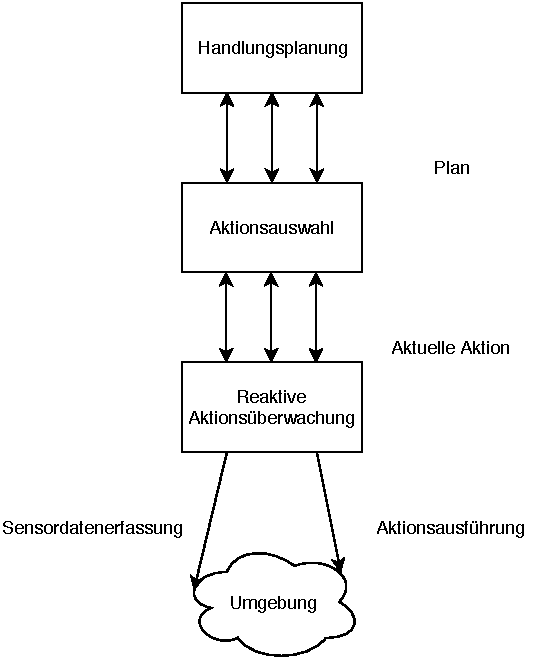
\includegraphics[scale=0.9]{Resources/PDF/HybridModel}
		\caption{Schema der Hybridmodell Schichten}
		\label{fig:PDF/HybridModel}
	\end{center}
\end{figure}
\begin{itemize}
	\item Die \textbf{Handlungsplanung} arbeitet auf hoher, strategischer Stufe in langen Zeitzyklen
	\item Die \textbf{reaktive Aktionsüberwachung} enthält die Verhaltensbausteine auf operativer Ebene, die in schellen Zeitzyklen die physische Roboteraktion anstoßen und überwachen
	\item die \textbf{mittlere Kontrollebene} hat die taktische Aufgabe, die jeweils \textbf{nächste Aktion aus dem Plan auszusuchen} zu instanzieren und auf die Ebene der Verhaltensbausteine zu zerlegen
	Des weiteren muss die die Rückmeldung von der Aktionsüberwachung interpretieren und entscheiden ob eine Aktion erfolgreich abgeschlossen ist. $\Rightarrow$ entscheiden ob die Handlungsplanung einen anderen Plan erstellen muss
\end{itemize}
\newpage
\paragraph{Kritik}
\begin{itemize}
	\item Mittlere Komponente benötigt den größten konzeptuellen und programmiertechnischen Aufwand
	\item Das mittlere Teilproblem ist deutlich komplexer als die beiden anderen
\end{itemize}
\subsection{Probabilistische Robotik}
\begin{itemize}
	\item Probabilistische Robotik berücksichtigt die \textbf{Unsicherheit der Wahrnehmund und der Aktionen}
	\item \textbf{Schlüsselidee} Information in Form von Wahrscheinlichkeitsdichten repräsentieren
	\item Eine Lokalisierung der Roboter wird unter Verwendung von wahrscheinlichkeitstheorie oder einer Wahrscheinlichkeitsverteilung eine Aussage über die Umgebung treffen
	\item \textbf{Probabilistische Wahrnehmung}: wenn man Sensorwerte schätzen kann, dann kann man mit Wahrscheinlichkeitstheorie/Wahscheinlichkeitsverteilung eine Aussage über die Umgebung treffen
	\item \textbf{Probabilistisches Handeln}: aufgrund der Unsicherheit über die Umgebung ist auch das Handeln mit Unsicherheit behaftet.
	Mit probabilistischen Ansätzen besteht die Möglichkeit Entscheidungen trotz Unsicherheit zu treffen
\end{itemize}
\paragraph{Vorteil} probabilistische Verfahren können auch mit weniger präzisen Umgebungsmodellen angewandt werden.
\paragraph{Nachteil} weniger effizient wegen komplexer Berechnungen, Approximation erforderlich
\subsection{Subsumption-Architektur in Bezug auf die Anforderungen des Robotersteuerungssystems}
\paragraph{Robustheit}
\begin{itemize}
	\item Wenn einige Steuerungsmodule ausfallen, arbeiten bei der Subsumption-Architektur in die restlichen Schichten einwandfrei $\Rightarrow$ \textbf{eingeschränktes, aber sinnvolles Verhalten möglich}
\end{itemize}
\paragraph{Unterschiedliche Ziele}
\begin{itemize}
	\item Mehrere Teilsituation können verschiedene Verhaltenselemente sinvoll machen, die sich widersprechen können.
	\item Die Wichtigkeit einer Handlung hängt vom Kontext ab, d.h. höhere Ziele können niederere Ziele ersetzen.
	\item Alle zu einem Zeitpunkt möglichen Verhaltenselemente werden parallel bearbeitet.
	\item Das \textbf{resultierende Verhalten wird in Abhängigkeit von Umwelteinflüssen dynamisch} bestimmt
	\item Das Gesamtergebnis hängt nicht von einer übergeordneten Instanz ab
\end{itemize}
\paragraph{Sensorwerte von mehreren Sensoren}
\begin{itemize}
	\item Der Roboter muss auch bei inkonsistenten Informationen eine Entscheidung fällen
	\item Die Subsumption-Architektur sieht keine zentrale Verarbeitung und Speichung der Umweltdaten
	\item Jedes Modul reagiert nur auf die Daten einzelner Sensoren, es muss \textbf{kein konsistentes Abbild der Umwelt erschaffen werden}
\end{itemize}
\paragraph{Erweiterbarkeit}
Das bestehende Verhalten kann jederzeit durch Hinzufügen weiterer Schichten um komplexere Funktionen erweitert werden
\section{ROS - Robot Operating System}
\subsection{Entwicklung}
\begin{itemize}
	\item \textbf{Das Architekturschema für Roboterkontrollsoftware} gibt es nicht $\Rightarrow$ deshalb heute auch Unterstützung der Roboter-Softwareentwicklung durch Middleware wie ROS
	\item \textbf{Zweck}: soll die Entwicklung von Software für Roboter vereinfachen und wiederkehrende Aufgaben standardisieren
	\item Standard für Robotoerkontrollsoftware
\end{itemize}
\subsection{Design Prinzipien}
\begin{figure}[H]
	\begin{center}
		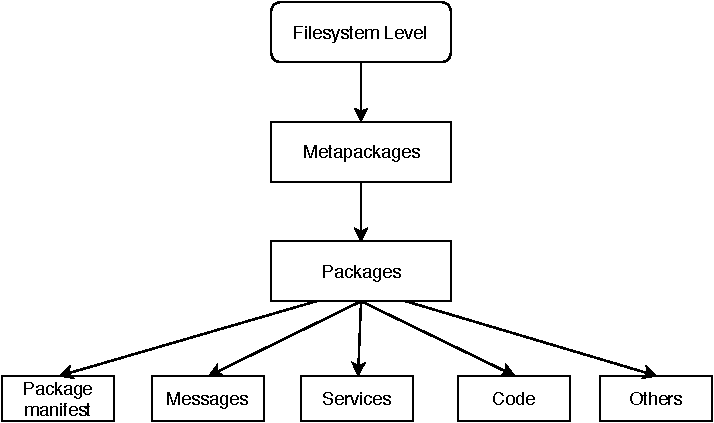
\includegraphics[]{Resources/PDF/FileSystem}
		\caption{Filesystem, das ROS zugrunde liegt}
		\label{fig:PDF/FileSystem}
	\end{center}
\end{figure}
\begin{itemize}
	\item Ein Package beinhaltet die ROS Prozesse, welche auch Nodes genannt werden
	\item Komplexe Prozesse werden durch Netzwerke von Nodes bewerkstelligt
	\item Roboterkontrollprogramm besteht aus vielen Prozessen, die potentiell über mehrere Rechner verteilt sein können
	\item Wichtigster Knoten ist der Master $\Rightarrow$ Abwicklung der internen Kommunikation
	\item Andere Knoten können nur starten, wenn ein Master existiert
	\item Nodes müssen sich beim Master anmelden
	\item Funktionalität (Kommandods, Ausführung v. Algorithemen) wird in eigenen Nodes realisiert
	\item Nodes sind in verschiedene Prozesse getrennt $\Rightarrow$ fehlerhafte Knoten hat i.d. Regel wenig Auswirkungen auf die anderen
	\item Knoten werden über Publish-Subscribe verknüpft
	\item \textbf{Asynchrone Nachrichten} werden durch Topics ausgetauscht
	\item \textbf{Synchrone Nachrichten} werden durch Services ausgetauscht
\end{itemize}
\subsection{Publish - Subscribe}
\paragraph{Nodes} sind Software-Module, die die Verarbeitung durchführen. Sie kommunizieren über Topics miteinander und tauschen dabei Nachrichten.
\paragraph{Kommunikation}
Die Kommunikation basiert auf einem \textbf{Publish Subscribe Pattern}
\begin{itemize}
	\item Wenn Daten weitergegeben werden sollen, wird ein Publisher erzeugt
	\item Publisher registriert sich beim Master und gibt Topics an
	\item Daten können in anderen Knoten abgerufen werden -- dazu wird ein (oder mehrere) Subscriber angelegt
	\item Subscriber frägt beim Master bezüglich gewünschten Topics an
	\item Daten werden über TCP/IP Sockets übertragen
\end{itemize}
\paragraph{Topics}
\begin{itemize}
	\item Themen, zu denen die Nodes Messages versenden
	\item Topics sind einfach Strings
	\item Verschiedene Nodes können zu einem bestimmten Topic Nachrichten versenden
	\item Ein Node kann sich prinzipiell zu mehreren Topics einschreiben und mehrere Topics publizieren
\end{itemize}
\paragraph{Services}
\begin{itemize}
	\item Nachteil von Publish Subscribe wird durch Services geschlossen
	\item Sind eine weitere Art, wie Nodes kommunizieren können
	\item Synchroner Nachrichtenaustausch mithilfe von Requests, welche von anderen Nodes mit einer Response beantwortet werden
	\item Ein Knoten registriert eine Aktion (Service), namentlich beim Master
	\item Ein Service Caller kann die Ausführung eines Services anstoßen, sobald dieser verfügbar ist
	\item geeignet für RMI oder einmalige Anfragen
\end{itemize}
\paragraph{Messages}
\begin{itemize}
	\item werden von Nodes bei der Kommunikation
	\item Messages sind streng typisierte, möglicherweise verschachtelte Datenstrukturen, die aus den primitiven Typen int, float, bool bestehen
	\item Eine Message kann andere Messages oder Felder von Messages enthalten
\end{itemize}
%seite 25 kapitel 2
\chapter{Lokalisation autonomer mobiler Robotersysteme}
\section{Abgrenzung: Lokalisation - Mapping - SLAM - Navigation}
\begin{itemize}
	\item \textbf{Lokalisation} Ermitteln der aktuellen Position des Roboters.
	\item \textbf{Kartenerstellung, Mapping oder Umgebungsmodellierung} hilft bei Entscheidung
	\subitem Kartenerstellung bedeuted die Auswertung der vom Roboter mittels Sensoren erfassten Daten der Umgebung mit dem Ziel, ein Umgebungsmodell zu erzeugne oder zu vervollständigen.
	\item \textbf{Großes Problem} Mapping
	\item \textbf{Pfadplanung oder Navigation} beantwortet die Frage \textbf{Wie gelange ich dorthin?} Bewegungsplanung oder Pfadplanung bedeutet die Berechnung der Fahrroute und der daraus abgeleiteten Bahn vom aktuellen Punkt zum Zielpunkt
	\item Man unterscheidet zwischen Navigation in unbekannter und in bekannter Umgebung.
	\item Selbstlokalisation und Kartenerstellung bedingen sich gegenseitig.
\end{itemize}
\section{Varianten der Selbstlokalisierung}
\paragraph{Lokale Selbstlokalisierung (position tracking)}
\begin{itemize}
	\item Die Startposition des Roboters ist ungefähr bekannt.
	\item Es handelt sich um \textbf{relative} Selbstlokalisierung
	\item Sobald sich der Roboter bewegt, muss aufgrund neuer Sensordaten die Position neu berechnet werden.
	\item Bezugspunkt ist der Startpunkt.
	\item \textbf{Methoden} Odometrie und Trägheitsnavigation
\end{itemize}
\paragraph{Globale Selbstlokalisierung}
\begin{itemize}
	\item Die Startposition ist unbekannt.
	\item Es handelt sich um \textbf{absolute Positionierung}
	\item An welcher Position der Roboter befindet, entscheidet er durch Auswerten seiner Sensordaten und durch erkennen von \textbf{signifikanten} Umgebungsmerkmalen
	\item \textbf{Mögliche Methode}: Triangulation
\end{itemize}
\paragraph{Kidnapped Robot Problem}
\begin{itemize}
	\item Die Position des Roboters ist anfangs bekannt
	\item Der Roboter wird willkürlich mit temporär deaktivierten Sensoren an eine beliebige andere Position versetzt, ohne darüber informiert zu werden.
	\item Auch dann muss das Verfahren robust die Position wiederfinden, zunächst muss der Roboter dies erkennen und sich dann relokalisieren
	\item Es muss eine erneute globale Lokalisierung durchgeführt werden
\end{itemize}
\section{Relative Lokalisierung versus Absolute Lokalisierung}
\paragraph{Relative Lokalisierung}
\begin{itemize}
	\item auch: \textbf{lokale}, \textbf{inkrementelle Lokalisierung} oder \enquote{tracking}
	\item Relativ zu einer Startpose wird sukzessiv die Änderung der Pose an diskreten, aufeinanderfolgenden Zeitpunkten ermittelt und integriert
\end{itemize}
\paragraph{Absolute Lokalisierung}
\begin{itemize}
	\item auch als \textbf{globale Lokalisierung} bezeichnet
	\item Die Pose wird in Bezug auf ein externes Bezugssystem ermittelt, z.B. einer Karte oder einem globalen Koordinatensystem
\end{itemize}
\paragraph{Ziel} Bestimme oder schätze die Position und Orientierung des Roboters in seiner Umgebung basieren auf
\begin{itemize}
	\item der Eigenbewegung
	\item durch Messungen der relativen Position zu unterscheidbaren Objekten in der Umgebung in Roboterkoordinaten (Ultraschall, Laser, Kamera)
\end{itemize}
%BSP Chapter 3 Seite 4 / 28 
\section{Transformation von Koordinatensystemen lokale <--> globale}
\paragraph{Kinematik} Die Kinematik ist die Lehre der Beschreibung von Bewegungen von Punkten im Raum. Dabei werden die Größen Weg, Geschwindigkeit und Beschleunigung betrachtet. Die Kinematik ist ein Teilgebiet der Mechanik.
\paragraph{Kinematische Robotermodell}
\begin{itemize}
	\item kreisförmiger Roboter
	\item Zweiradantrieb
	\item Bewegung in der Ebene
\end{itemize}
\paragraph{Lokales Koordinatensystem}
\begin{itemize}
	\item mit dem Roboter verbunden
	\item Ursprung in der Mitte der Antriebsachse
	\item x-Achse zeigt in Richtung des Roboterfrontteils
\end{itemize}
\paragraph{Festlegung der Roboterposition im globalen Koordinatensystem}
\begin{itemize}
	\item durch die Koordinaten $M(x_{M}, y_{M})$ im globalen Koordinatensystem
	\item durch den Winkel $\theta$ zwischen der lokalen x-Achse und der globalen x-Achse
	\item Pose p gegeben durch: p = $(x_M, y_M, \theta)^{T}$
\end{itemize}
\paragraph{Transformation von lokalen in globale Koordinaten}
\begin{itemize}
	\item Koordinaten von P im lokalen Koordinatensystem: $p_l=(x_l, y_l)^T$
	\item Koordinaten von P im globalen Koordinatensystem: $p_g = (x_g, y_g)^T$
	\item Transformation von $p_l$ nach $p_g(m=(x_M, y_M)^T: p_g=R(\theta)p_l)$
\end{itemize}
\paragraph{Transformation von globalen in lokale Koordinaten}
\begin{itemize}
	\item Transformation von globalen in lokale Koordinaten $p_l = R(\theta)^-1(p_g - m) = R(-\theta)(pg - m)$
\end{itemize}
\section{Karten für statistische und dynamische Umgebungen}
\begin{itemize}
	\item Generell gilt: \textbf{Karten} sollen eine explizite Repräsentation des Raumes sein.
	\item Die Karten sind auf die Sensorik des Roboters zugeschnitten
	\item Die Karten sind nicht vorrangig für den menschlichen Betrachter bestimmt, sondern der Roboter soll sie effizient nutzen können.
\end{itemize}
\paragraph{Statische Umgebungen}
\begin{itemize}
	\item basierend auf der Annahme, dass sich zwar der Zustand des Roboters innerhalb der Umgebung, nicht jedoch die Umgebung selbst ändert.
	\item Karte spiegelt die wirkliche Umgebung wider.
\end{itemize}
\paragraph{Dynamische Umgebungen}
\begin{itemize}
	\item Objekte können ihre Lage oder ihren Zustand ändern
	\item In der Karte registrierte Objekte können verschwinden, nicht registrierte Objekte auftauchen
	\item \enquote{Lernende} Karten sind ein fundamentales Problem in der mobilen Robotik
\end{itemize}
\subsection{Mapping Methoden}
\paragraph{Weltzentriert}
\begin{itemize}
	\item Die Pose aller Objekte einschließlich des Roboters werden in der Umgebung in Bezug auf ein festes Koordinatensystem repräsentiert.
	\item \textbf{Indoor}: Ursprung kann eine Zimmerecke sein
	\item \textbf{Outdoor}: Benötigung eines globalen Koordinatensystems, wie z.B. die Längen- oder Breitengrade, i.d.R. nutzen von \textbf{WGRS}(World Geographic Reference System)
\end{itemize}
\paragraph{Roboterzentriert} gebraucht um bspw. Kollisionen zu vermeiden
\begin{itemize}
	\item Durch Koordinaten-Transformation kann zwischen den verschiedenen Referenz-Frames konvertiert werden
\end{itemize}
\subsection{Arten von Modellen}
\begin{itemize}
	\item Die wichtigste Form von Umgebungsmodellen für mobile Roboter sind Umgebungskarten.
	\item Die folgende Ausführungen beziehen sich auf geeignet Karten für \textbf{mobile, autonome Landfahrzeuge}
\end{itemize}
\begin{figure}[H]
	\begin{center}
		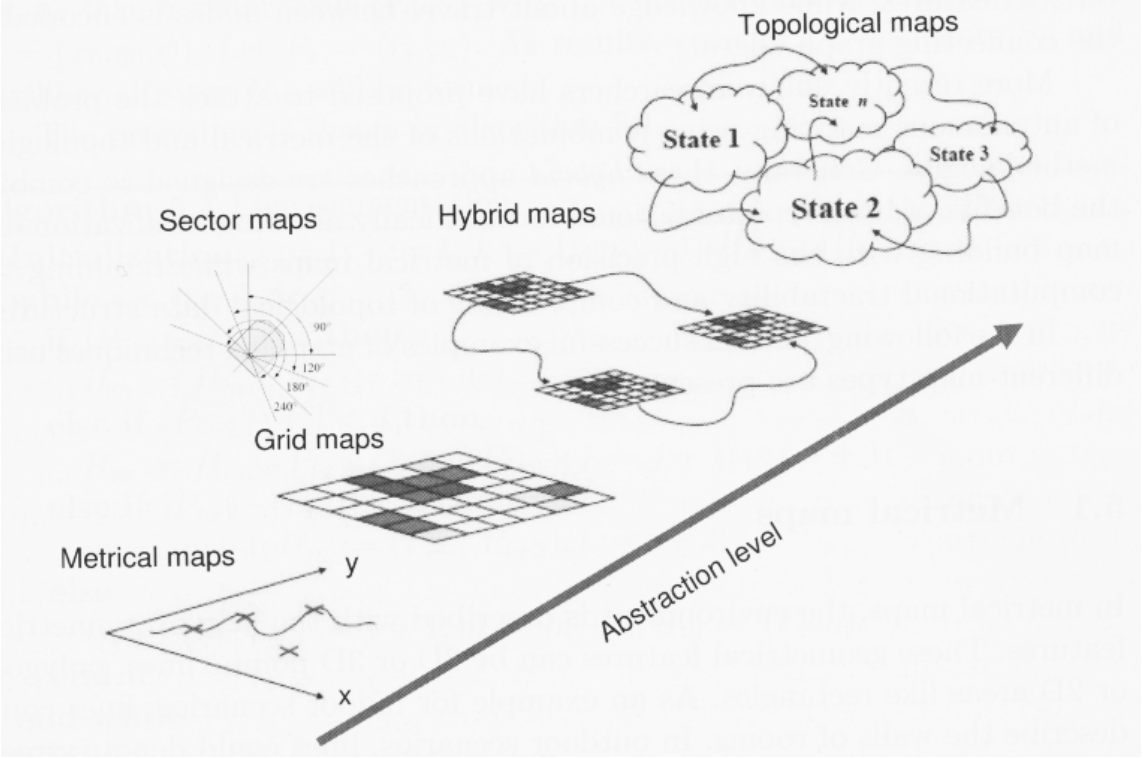
\includegraphics[scale=0.42]{Resources/PNG/MapTypes.PNG}
		\caption{}
		\label{fig:PNG/MapTypes.PNG}
	\end{center}
\end{figure}
\paragraph{Arten von Umgebungsmodellen}
\begin{itemize}
	\item \textbf{kontinuierliche metrische Karten}, zweidimensional oder dreidimensional:
	\subitem jedes Objekt wird assoziiert mit Koordinaten
	\item \textbf{diskrete metrische Karten, Grid Maps}, zweidimensional oder dreidimensional:
	\subitem der Raum wird gleichmäßig oder ungleichmäßig aufgeteilt; Objekte werden mit Positionen innerhalb des Gitters assoziiert
	\item \textbf{Hybrid Maps}
	\item \textbf{Topologische Modelle} nur zweidimensional
	\subitem im Vordergrund steht die Beziehung der Objekte zueinander
\end{itemize}
\subsection{Kontinuierliche Metrische Karten}
\begin{itemize}
	\item Metrische Lokalisierung, beruht auf Ultrashall oder Laserscannern
	\item Exakte Beschreibung der Umgebung mit 2D oder 3D Modellen möglich
	\item Die Positionen von Objekten der Umgebung werden durch ein Koordinatensystem repräsentiert.
	\item \textbf{Vorteil}: detailliertes Bild der Umgebung
	\item \textbf{Nachteil}: große, unstrukturierte Datenmengen erschweren die Pfadplanung
\end{itemize}
\subsection{Grid Maps - Rasterkarten}
\begin{itemize}
	\item Die Umwelt des Roboters wird in ein gleichmäßiges Raser oder Grid zerlegt.
	\item Jede Zelle enthält den Belegtheitsgrad der Zelle $\Rightarrow$ zeigt an ob zelle mit einem Hindernis belegt ist oder nicht
	\item Verschiedene Modelle verwenden unterschiedliche Werte
	\subitem zwei Werten
	\subitem freie Zellen, belegte Zellen und Zellen mit Mischbelegung
	\subitem Prozentsatz der Belegungswahrscheinlichkeit
	\item Notwendige Informatinoen sind z.B.:
	\subitem x, y als Koordinaten (Zeile, Spalte) einer Zelle
	\subitem Sensordaten des Roboters
	\subitem ein boolscher Wert für den Zustand der Zelle
	\item Die Werte in den Zellen sind unabhängig voneinander
	\item Eine Steigerung der Messgenauigkeit der Sensoren führt dazu, dass die Rasterelemente immer kleiner werden
	\item Für eine kompakte Notation können Grid Maps im 2-dimensionalen Raum mit Quadtrees im 3-dimensionalen mit Octtrees gespeichert werden
\end{itemize}
\paragraph{Gleichmäßige Gitterstruktur vs. Adaptiver Gitterstruktur}
\begin{figure}[H]
	\begin{center}
		\includegraphics[scale=0.5]{Resources/PNG/Quadtrees.PNG}
		\caption{}
		\label{fig:PNG/Quadtrees.PNG}
	\end{center}
\end{figure}
\begin{itemize}
	\item links oben zeigt die Objekte in einer gleichmäßigen Gitterstruktur
	\item rechts oben zeigt die zugehörige Repräsentation über Belegtheiten der Zellen
	\item speicherintensiv bei gleichmäßiger Unterteilung des Raums $\Rightarrow$ adaptive Unterteilung des Raums und Speicherung in Quadtrees oder bei 3. Dimension Octtrees
\end{itemize}
\subsection{Adaptive Unterteilung}
\begin{itemize}
	\item Ausgangszustand: Rechteck mit Hindernissen
	\item Fläche wird unterteilt in 4 Rechtecke gleicher Größe
	\item Jedes Rechteck wird rekursiv wieder in 4 Rechtecke unterteilt $\Rightarrow$ Quadtree
	\item Attributierung der Knoten:
	\subitem \textbf{Frei}: Rechteck enthält keinen Teil eines Hindernisses
	\subitem \textbf{Belegt}: Rechteck ist vollständig von Hindernis belegt
	\subitem \textbf{Gemischt}: Rechteck enthält Punkte, die zu einem Hindernis gehören, sowie solche die es nicht tun
	\item Nur gemischte Knoten werden weiter unterteilt
\end{itemize}
\paragraph{Vorteile} schnell und leicht feststellbar, ob Punkt in einem Hindernis liegt
\paragraph{Nachteile} 
\begin{itemize}
	\item Konturen der Objekte und der Freiraum zwischen ihnen wird unpräzise repräsentiert
	\item Um die Datenfülle zu reduzieren, wird das Raster zu grob gewählt und dadurch ein möglicher Weg durch Mischpixel versperrt
\end{itemize}
\paragraph{Weiterer Verwendungszweck}
Neben der reinen Lokalisierung können die Karten auch dazu verwendet werden eine Fahrspur (Trakektorie) zu berechnen.
\begin{figure}[H]
	\begin{center}
		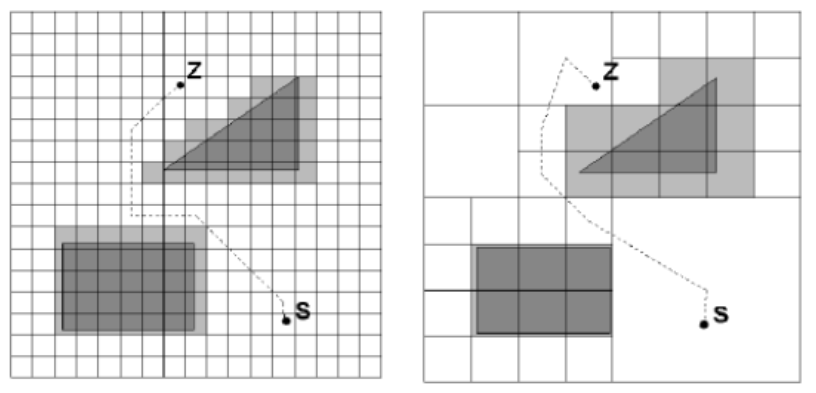
\includegraphics[scale=0.5]{Resources/PNG/Trajektorie}
		\caption{}
		\label{fig:PNG/Trajektorie}
	\end{center}
\end{figure}
\subsection{Weitere Beispiele für Umgebungskarten}
\begin{itemize}
	\item Laserscan Karten
	\item Bildbasierte Karten
\end{itemize}
\subsection{Topologische Karten}
Bedingt geeignet zur Lokalisation, Haupteinsatzgebiet ist die Pfadplanung.
\begin{figure}[H]
	\begin{center}
		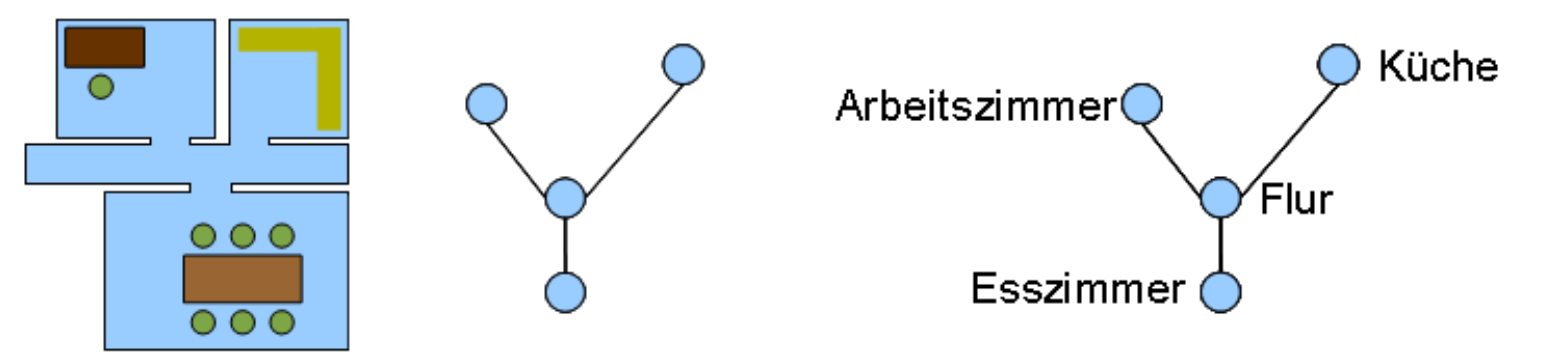
\includegraphics[scale=0.42]{Resources/PNG/TopologischeKarte.PNG}
		\caption{}
		\label{fig:PNG/TopologischeKarte.PNG}
	\end{center}
\end{figure}
\begin{itemize}
	\item Modelle bilden einen \textbf{Graphen}
	\item \textbf{Knoten} entsprechen Orten oder Bereichen der Umgebung
	\item Beziehungen zwischen den Orten werden durch \textbf{Kanten} modelliert.
	\item Zwei Knoten sind durch eine Kante verbunden, wenn sie unmittelbar voneinander erreichbar sind.
	\item \textbf{Gewichte}: Maß für die Länge der Wege
	\item Ist die Länge der jeweiligen Wegstücke bekannt, lässt sich der kürzeste Weg finden.
\end{itemize}
\paragraph{Vorteile}
\begin{itemize}
	\item Kompaktheit
	\item Gute Skalierbarkeit für welträumige Umgebungen.
	\item Es gibt viele schnelle Algorithemn auf Graphen, die gut zur Pfadplanung eingesetzt werden können
\end{itemize}
\paragraph{Nachteil} Relevante Umgebungsmerkmale werden verdeckt. Landmarken werden schwerer erkannt.
\subsection{Hybrid Maps}
\begin{itemize}
	\item Kombinieren metrische und topologische Ansätze
	\item Ermöglichen Lokalisation und Kantenerstellung mit hoher Präzision
	\item Erhalten die Kompaktheit der topologischen Ansätze
\end{itemize}
\paragraph{Abstraktions-basierter Ansatz}
\begin{itemize}
	\item Basis: konstruieren einer metrischen Karte der Umgebung
	\item $\Rightarrow$ aufbau einer kompakten topologischen Repräsentation
	\item \textbf{Vorteil} Effizient Planung eines Pfads zu einem gegebenen Ziel aufgrund der Abstraktion.
	\item Die zugrunde liegende metrische Karte wird für Relokalisation und Hindernisvermeidung benötigt.
\end{itemize}
\section{Passive und Aktive Selbstlokalisierung}
\subsection{Passive Verfahren}
\begin{itemize}
	\item bestimmen oder schätzen die Roboterposition mittels aktueller Sensorinformationen
	\item beeinflussen \textbf{nicht} die Bewegung und Orientierung des Roboters
	\item Lokalisierungsmodul beobachtet nur die Roboteroperationen
	\item Roboter bewegt sich zufällig hin und her bzw. führt die zu erledigende Aufgabe durch
\end{itemize}
\subsection{Aktive Verfahren}
\begin{itemize}
	\item besitzen vollständige oder teilweise Kontrolle über die Bewegungen des Roboter und Ausrichtung der Sensoren
	\item fähhrt gezielt bestimmte Orte an um Mehrdeutigkeiten zwischen mehreren Orten aufzulösen
\end{itemize}
\section{Landmarken}
\subsection{Definition}
\begin{itemize}
	\item Als Landmarken werden \textbf{eindeutig identifizierbare Charakteristiken der Umwelt} bezeichnet, die von entsprechenden Sensoren erkannt werden können.
\end{itemize}
\paragraph{Landmarke}
\begin{itemize}
	\item ihre Position im Weltmodell ist bekannt
	\item sichtbar von unterschiedlichen Positionen aus
	\item erkennbar unter verschiedenen Belichtungen und Blickwinkeln
	\item relative Position bestimmbar
	\item stationär, oder dem Navigationsmechanismus musss die Bewegung bekannt sein
\end{itemize}
\paragraph{Vorteil} Navigation erfolgt mit der Umwelt selbst und nicht mittels erechneter Daten
\subsection{Natürliche Landmarken}
\begin{itemize}
	\item Werden nicht zum Zweck der Positionsbestimmung aufgestellt, können aber dafür verwendet werden
	\item Grundsätzlich Passiv
\end{itemize}   
\subsection{Künstliche Landmarken}
\begin{itemize}
	\item Markante Objekte, eigens zum Zwech der Positionsbestimmung in der Umgebung installiert.
\end{itemize}





































\chapter{Fortbewegung, Lokalisierungsalgorithmen}
\section{Relative Lokalisierung}
\subsection{Dead Reckoning}
\begin{itemize}
	\item \textbf{Koppelnavigation oder Dead Reckoning} ursprünglich in der Nautik verwendet
	\item Mathematisches Verfahren - \textbf{Vorwärtskinematik} - zur Positionsbestimmung
	\item Ausgehend von einer Startposition ist es dem Navigator möglich, seine \textbf{aktuelle Position zu berechnen} aufgrund der \textbf{zurückliegenden bekannten Kurs- und Geschwindigkeitswerte}
\end{itemize}
\begin{figure}[H]
	\begin{center}
		\includegraphics[scale=0.7]{Resources/PDF/deadreckoning.pdf}
		\caption{}
		\label{fig:PDF/deadreckoning.pdf}
	\end{center}
\end{figure}
\begin{itemize}
	\item A sei ein gegebener Ausgangspunkt
	\item Radius wird angegeben der zur Abweichung proportional ist, bsp. hier 0,5m.
	\item Der Radius spiegelt die mit der Zeit kumulierte Ungenauigkeit wieder
	\item Eine mögliche Roboterposition ist dann innerhalb des Sektors gegeben der durch die Linien eingegrenzt wird
\end{itemize}
\paragraph{Vorteile}
\begin{itemize}
	\item einfache Implementierung
	\item leichte Interpretation der Daten
	\item unkomplizierte Bedienung
	\item passable Kurzstreckengenauigkeit
\end{itemize}
\paragraph{Nachteile}
\begin{itemize}
	\item Startposition muss bekannt sein
	\item Genauigkeit nimmt mit zunehmender Länge der befahrenen Strecke drastisch ab
\end{itemize}
\subsection{Odometrie}
Odometrie ist die Wissenschaft der Positionsbestimmung eines Fahrzeugs durch die Beobachtung seiner Räder.
\paragraph{Grundlegendes verfahren}
\begin{itemize}
	\item Sensoren an Rädern messen Drehbewegung
	\item \textbf{Relative Positionsbestimmung:} Die \textbf{Bestimmung der Position} erfolgt ausgehend von einer bekannten Position durch Berechnung des zurückgelegten Weges und anhand von Daten über den Roboter selbst.
	\item Es wird Inkrementalgebern die Anzahl $n$ der Radumdrehungen zwischen zwei Messpunkten gezählt. Aus dem bekannten Radumfang wird die wegdifferenz berechnet mit:
	\subitem $\Delta = \Pi \times d \times n $
	\item \textbf{Ausrichtung} kann durch differentiale Odometrie erfolgen: es werden z.B. die unterschiedlichen Entfernungen gemessen, die die linken und rechten Räder zurückgelegt haben.
\end{itemize}
\paragraph{Vorteile}
\begin{itemize}
	\item kostengünstig
	\item hohe Abtastraten
	\item passable Kurzzeitgenauigkeit
\end{itemize}
\paragraph{Fehlerquellen}
\begin{itemize}
	\item Fehlerhafte Messung des Raddurchmessers
	\item Raddurchmesser nicht gleich, Unrundheit des Radess
\end{itemize}
\paragraph{Fehlerberücksichtigung}
\begin{itemize}
	\item Die \textbf{Fehler} fließen in die Positionsdifferenz ein, werden zur letzten bekannten Position hinzuaddiert und \textbf{summieren sich mit jedem Messschritt}
	\item Fehlerellipse wächst mit zurückgelegtem Weg
	\item Odometrie als alleiniges verfahren nur für kurze Strecken geeignet
	\item Fehler lassen sich bei geringen Geschwindigkeiten und geringer Beschleunigung reduziern
\end{itemize}
\subsection{2D-Scanmatching}
\begin{itemize}
	\item Ausgangslage sind zwei Scans, ein Scan M (\textbf{Modell}) und ein zweiter Scan D (\textbf{Daten})
	\item Es wird eine Transformation des einen Scans berechnet und zwar so, dass beide optimal überlagert werden
	\item Die Transformationen bestehen nur aus einer Rotation und einer Translation
	\item Die Überlagerung ist optimal, wenn Punkte, die in der realen Szene nahe beieinander liegen, auch in den registrierten Messdaten nahe beieinander liegen.
	\item \textbf{Ziel}: Fehlerfunktion minimieren $\Rightarrow$ Abstände der Punkte des einen Scans zu ihren korrespondierenden Punkten des zweiten Scans
	\item Die Transformation des zweiten Scans entspricht dann der Bewegung des Roboters zwischen der Aufnahme der Daten; durch sukzessiven Vergleich kann damit die Bewegung des Roboters nachverfolgt werden
\end{itemize}
%TODO Rework this after understanding it
\paragraph{Iteratives Vorgehen}
\begin{figure}[]
	\begin{center}
		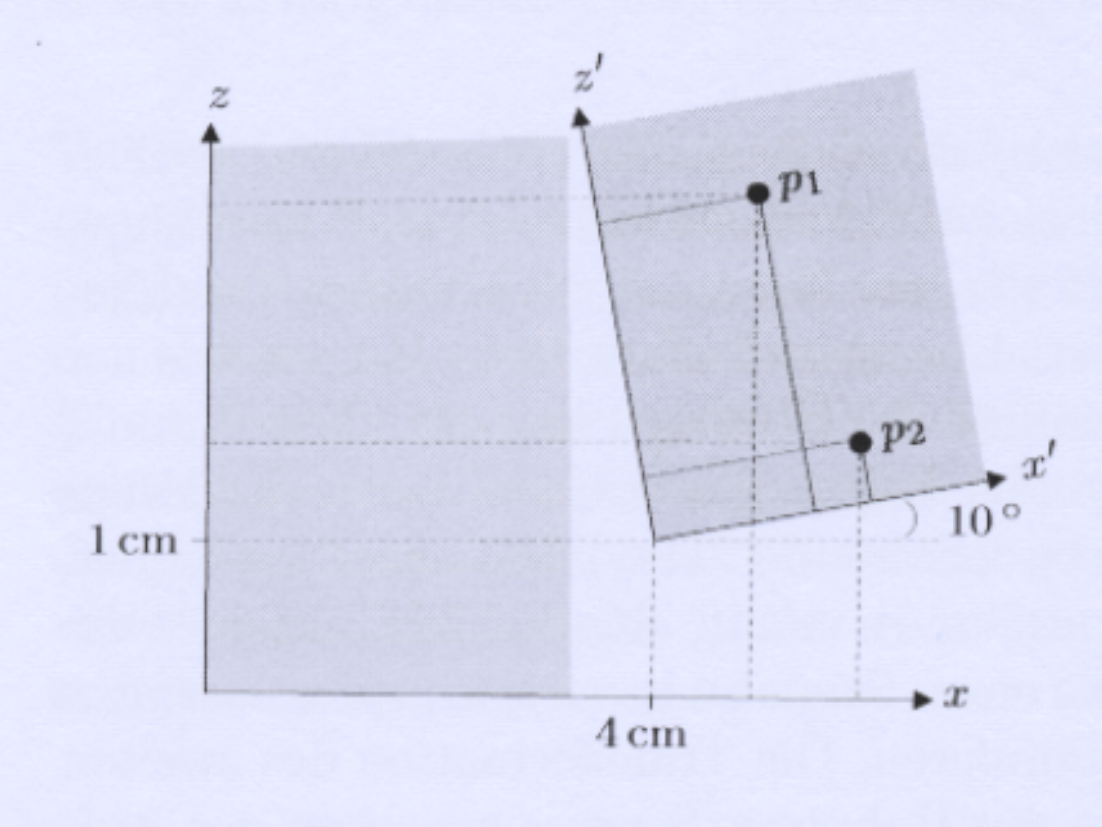
\includegraphics[scale=0.3]{Resources/PNG/2DScan.PNG}
		\caption{}
		\label{fig:PNG/2DScan.PNG}
	\end{center}
\end{figure}	
\begin{itemize}
	\item \textbf{Annahme:} die korrespondierenden Punkte sind bekannt $\Rightarrow$ eine \textbf{Transformation} kann berechnet werden, die diese Mengen aufeinander abbildet
	\item \textbf{Beispiel} zwei Scans mit einer Poseänderung des zweiten um $(4cm, 1cm, 10 \deg)^T$ beide Scans sehen dieselben Raumpunkte p1 und p2
	\item Obige Annahme i.d.r. nicht erfüllt $\Rightarrow$ \textbf{nicht eindeutig zu bestimmen, welche Punkte zwischen den beiden Scans korresponideren}
	\item \textbf{Lösung}: \textbf{iteratives Vorgehen}, bei dem zunächst eine \textbf{Schätzung} der Punktepaarung stattfinden und die Pose des zweiten Scans unter dieser Paarung optimiert wird.
	\item Iterativ werden mit dem transformierten Scan neue Punktepaare berechnet, bis ein Abbruchkriterium erfüllt ist, d.h. bis sich die Transformation zwischen zwei Schritten nich mehr signifikant ändert
\end{itemize}
\paragraph{Transformationsberechnung}
\begin{itemize}
	\item \textbf{Gesucht}: Mögliche Menge von Translationen und Rotationen, unter denen ein korrektes Matching möglich ist.
	\item $(t_x, t_z, \theta)^T$, die eine Translation um $t_x$ in x-Richtung und $t_z$ entlang der Z-Achse durchführt, sowie eine Rotation um den Winkel $\theta$
	\item Der Scan M besteht aus einer Menge von Punkten ($m_i$)i=1,2...N
	\item Der Scan D besteht aus einer Menge von Punkten ($D_i$)i=1,2...N
\end{itemize}
\paragraph{Minimum der Funktion}
$E(\theta, t)=\sum_{i=1}^{N}\left\|p_{i}-\left(\boldsymbol{R}_{\theta} \boldsymbol{p}_{i}^{\prime}+\boldsymbol{t}\right)\right\|^{2}$
\paragraph{Transformation zur mimierung der Fehlerfunktion E}
Folgende Transformation mit ggb. Parametern minimiert die Fehlerfunktion:\\
$\theta=\arctan \left(\frac{S_{z x^{\prime}}-S_{x z^{\prime}}}{S_{x x^{\prime}}+S_{z z^{\prime}}}\right)$
\\
Hierbei ist \\
$t_{x}=c_{x}-\left(c_{x}^{\prime} \cos \theta-c_{z}^{\prime} \sin \theta\right)$ und \\
$t_{z}=c_{z}-\left(c_{x}^{\prime} \sin \theta+c_{z}^{\prime} \cos \theta\right)$
%TODO Look at BSP 26 / 28



\chapter{Navigation}
\section{Bekanntes vs. unbekanntes Terrain}
Man unterscheidet zwischen Algorithmen für:
\begin{itemize}
	\item \textbf{bekannte Umgebungen} (auch während der Fahrt ändert sich die Umgebung nicht)
	\item \textbf{unbekannt Umgebung}
\end{itemize}
\begin{itemize}
	\item Gebiet \textbf{vollständig bekannt} $\Rightarrow$ Lösung der Suche mittels eines Graphen.
	\item \textbf{unvollständig oder gar nicht bekanntes Gelände} $\Rightarrow$ Berechnungen erfolgen auf \textbf{lokalen Teilinformationen}
	\subitem Neue Informationen $\Rightarrow$ \textbf{inkrementelle Anpassung} über Sensoren
\end{itemize}
\section{Navigation in unbekanntem Terrain}
\subsection{Konturverfolgung}
\begin{itemize}
	\item Eine \textbf{Freiraumfahrt} d.h. eine Fahrt durch ein Gelände, dessen Raum möglichst weit und frei von Hindernissen ist $\Rightarrow$ nicht immer Zielführend
	\item Lösung: \textbf{Konturverfolgung}
	\subitem Roboter wird nah an einem Objekt (Wand, Hinderniss) entlang bewegt
	\subitem Es sollte möglichst ein gegebener Abstand $d$ eingehalten werden
\end{itemize}
\newpage
\paragraph{Regelung des Abstands d}
\begin{lstlisting}
IF (Distance to Wall > d) 
	THEN turn to wall

IF (Distance to Wall < d) 
	THEN turn away from wall

IF (Distance to Wall == d) 
	THEN Drive straight ahead
\end{lstlisting}
\subsection{Sensorbasierte Planer - Navigation mit Hinderniskontakt}
\paragraph{Bug1 Algorithmus}
Fordert zwei bestimmte Verhalten:
\begin{itemize}
	\item bewege dich auf einer geraden Linie
	\item folge einer Begrenzung in einem bestimmten Abstand
\end{itemize}
\begin{figure}[H]
	\begin{center}
		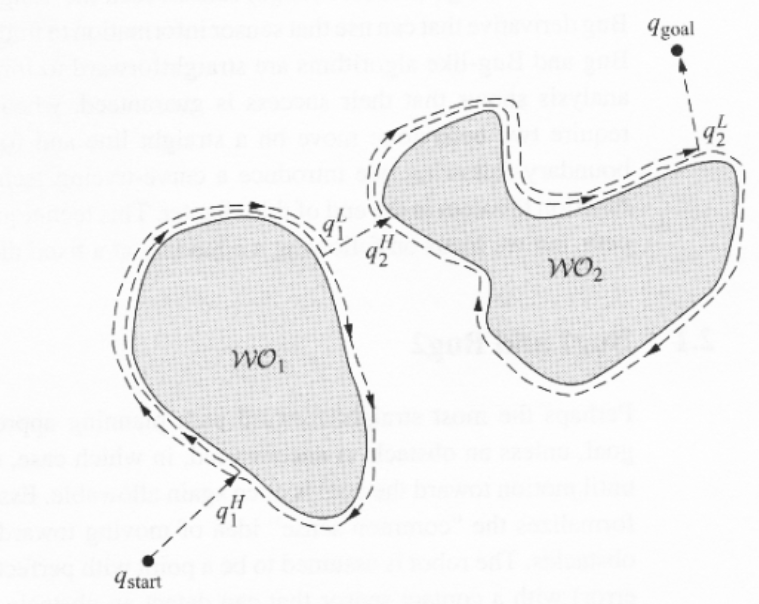
\includegraphics[scale=0.5]{Resources/PNG/Bug1.png}
		\caption{Bug1 Algorithmus Route}
		\label{fig:PNG/Bug1.png}
	\end{center}
\end{figure}
\paragraph{Vorraussetungen}
\begin{itemize}
	\item Roboter benötigt einen Sensor zur Erkennung eines \enquote{Kontakts} mit einem Hindernis
	\item Roboter kann die Distanz zwischen zwei Punkten x und y messen
	\item der Arbeitsraum ist begrenzt
\end{itemize}
\paragraph{Algorithmus}
\begin{itemize}
	\item Roboter folgt Linie zum Ziel bis er beim Punkt $q_1^H$ auf ein Hinderniss trifft
	\item Roboter umfährt das Hindernis bis er erneut beim gleichen Punkt auf das Hindernis trifft
	\item Roboter bestimmt den nähesten Punkt (Leavepoint) $q_1^H$ vom Hindernis zum Ziel und fährt diesen Punkt an
	\item Von diesem Punkt fährt der Roboter geradewegs zum Ziel bis er das Ziel erreicht oder erneut auf ein Hindernis trifft
\end{itemize}
\paragraph{Exception}
Schneided die Linie von $q1^L$ zum Ziel das \textbf{akutelle Hindernis} gibt es keine Lösung
\begin{figure}[H]
	\begin{center}
		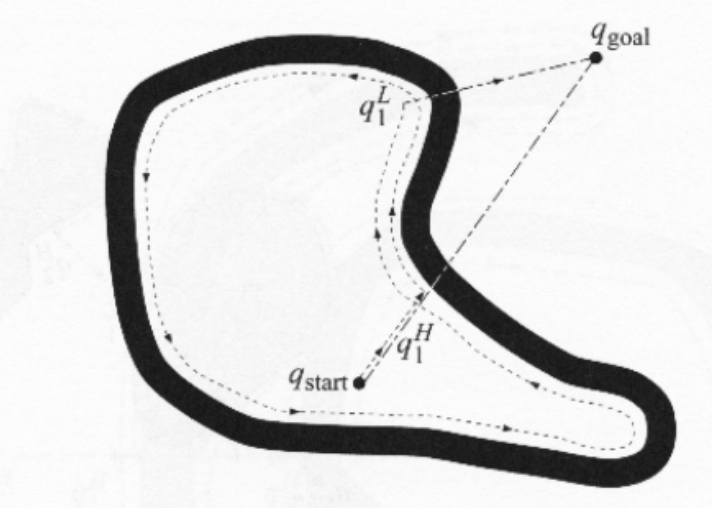
\includegraphics[scale=0.4]{Resources/PNG/Exception1.PNG}
		\caption{}
		\label{fig:PNG/Exception1.PNG}
	\end{center}
\end{figure}
\paragraph{Bug2-Algorithmus}
\textbf{Idee:}
\begin{itemize}
	\item Linie vom Start $S$ zum Ziel $T$ konstruieren
	\item bewegt sich möglichst auf dieser Linie
	\item Roboter trifft auf Objekt $\Rightarrow$ umfahren in einer bestimmten Richtung bsp. immer rechts herum
	\item Hindernis wird solange umfahren, bis der Roboter wieder auf einen Punkt auf der Linie $ST$ trifft, der näher zum Ziel liegt als der ursprüngliche Kontaktpunkt mit dem Hindernis
\end{itemize}
\textbf{Algorithmus}:
\begin{lstlisting}
1. Auf Geraden ST in Richtung T fahren bis:
	a.) Ziel erreicht wird --> END
	b.) Hinternis getroffen wird --> Schnittpunt Hj setzen
		--> Schritt 2
2. Umfahre das Objekt bis:
	a.) das Ziel erreicht wird --> END
	b.) Gerade ST in einem Punkt Q getroffen wird mit Strecke QT kleiner als Strecke HjT
		QT wird in Richtung T verlassen
		Q als Leavepount Lj setzen
		i um 1 erhoehen
		--> Schritt 1
	c.) zum letzten Hitpoint Hj zurueckgekehrt wird
		Algorithmus wird abgebrochen
		Es gibt keinen Weg zu T
\end{lstlisting}
\begin{itemize}
	\item Ev. wird kein Weg zum Ziel gefunden
\end{itemize}
\begin{itemize}
	\item Bei Komplexen Hindernissen kann Ziel mit \textbf{Backtracking} gefunden werden
\end{itemize}
\paragraph{Bug3-Algorithmus}
\begin{figure}[H]
	\begin{center}
		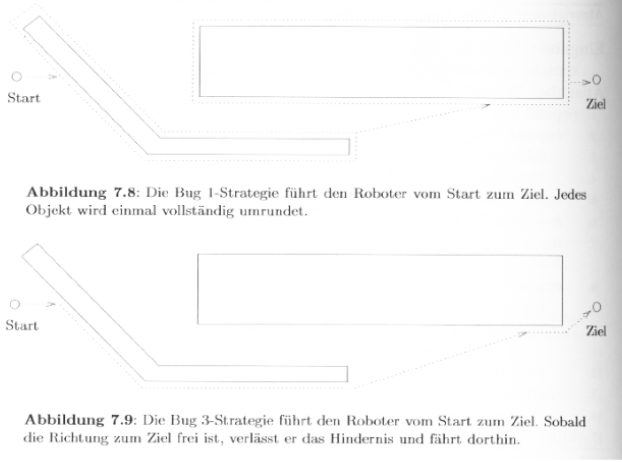
\includegraphics[scale=0.6]{Resources/PNG/Bug3.PNG}
		\caption{}
		\label{fig:PNG/Bug3.PNG}
	\end{center}
\end{figure}
\subsection{Labyrinthe}
\paragraph{Grundprobleme}
\begin{itemize}
	\item Es wird davon ausgeangen, dass der Roboter berühren oder \enquote{sehen} kann
	\item Zwei grundlegend Hauptprobleme:
	\subitem Einen \textbf{Weg in ein Labyrinth} finden, um einen bestimmten Gegenstand oder \textbf{Schatz zu erreichen} sowie den \textbf{Rückweg zum Eingang}
	\subitem \textbf{Flucht aus einem Labyrinth} von einer unbekannten Stelle aus.
	\item Enger Zusammenhang zwischen Labyrinth und Graphen $\Rightarrow$ Jeder Korridor:= Kante und jede Kreuzung:= Knoten
	\subitem Bei bekanntem Labyrinthe $\Rightarrow$ Suchproblem auf in Bäumen
\end{itemize}
\paragraph{Verlassen eines Labyrinths mit Pledge Algorithmus}
\textbf{Grundidee}: Vorsichtig geradeaus bis man auf ein Hindernis trifft und dann mit der \enquote{linken} Hand immer an der Wand entlang bis zum Ausgang.\\
\textbf{Problem}: Enthält das Labyrinth eine Säule, läuft man für immer im Kreis
\begin{itemize}
	\item \textbf{Lösung} $\Rightarrow$ man folgt der Wand nur solange, bis man wieder in die alte Richtung schaut.
\end{itemize}
\textbf{Allgemeingültige Lösung}: Drehungen beim Abbiegen an den Ecken mitzählen.
Bei jeder Linksdrehung wird der Umdrehungszähler inkrementiert, bei jeder Rechtsdrehung dekrementiert.
\begin{itemize}
	\item Bewege den Roboter geradeaus bis eine Wand erreicht ist
	\item Folge der Wand bis Umdrehungszähler 0 ist
\end{itemize}
\paragraph{Verlassen eines Labyrinths mit Ariadnefaden}
\begin{itemize}
	\item \textbf{Ziel}: einen Weg zu einem versteckten Ziel im Labyrinth sowie wieder zurück zum Eingang finden ohne dass eine Karte des Labyrinths bekannt ist
	\item \textbf{Idee}: Wenn man ein Labyrinth betritt Faden ausrollen $\Rightarrow$ zurückverfolgen bringt einen zurück zum Eingang.
\end{itemize}
\textbf{Vorraussetzungen und grundsätzliches Vorgehen}
\begin{itemize}
	\item einer Wand folgen
	\item Umdrehen
	\item Kreuzungen erkennen
	\item Ziel erkennen
	\item Faden auslegen und wieder einsammeln
	\item Faden am Boden erkennen
	\item Faden zur nächsten Kreuzung folgen
\end{itemize}
\paragraph{Tarry und Tremaux Algorthmus}
\begin{itemize}
	\item Beispiel für klassische Tiefensuche
	\item Richtung, in der sich das zu suchende Objekt befindet ist unbekannt.
	\item Graph kann zyklen enthalten
	\item Es wird ein zyklisch gerichteter Graph durch jede Kante konstruiert, wobei jede Kante nur einmal pro Richtung besucht wird
\end{itemize}
\textbf{Algorithmus:}
\begin{itemize}
	\item Starte willkürlich an einem Knoten
	\item Folge einem möglichen Pfad, markiere die Kante, in welcher Richtung sie betreten worden ist
	\item Sind alle Kanten schon betreten, eine auswählen, die bis jetzt nur in die Gegenrichtung betreten wurde.
	\item Trifft man auf eine Sackgasse oder einen schon besuchten Gang, zurück zur letzten Kreuzung
	\item Es darf kein Pfad betreten werden, der schon in beide Richtungen besucht wurde.
	\item Algorithmus ist beendet, wenn der Startpunkt erreicht wird.
\end{itemize}
\section{Pfadplanung für mobile Roboter in bekanntem Terrain}
\subsection{Bewegungsplan für mobile Roboter}
Ziel der Navigation ist es, ein Fahrzeug in der Umwelt zu bewegen.
Dies beinhaltet drei Unteraufgaben:
\paragraph{Globale Pfadplanung}
\begin{itemize}
	\item \textbf{Vorraussetzung}: es gibt eine Karte
	\item suche eines Pfades von einem Start- zu einem Zielpunkt in vorhandenem Umgebungsmodell
	\item evtl. auch Suche nach Pfad mit geringsten Kosten
	\item Kompletter Pfad beschrieben durch Menge von Punkten
\end{itemize}
\paragraph{Lokale Pfadplanung} berücksichtigt Fahrzeug-Dimension und kinematische Einschränkungen
\paragraph{Path Control} generiert geeignet Steuerbefehle, um den vorberechneten Pfad zu folgen
\subsection{Konfigurationsraum}
\paragraph{Herleitung}
\begin{itemize}
	\item Abmesungen, Form, Bewegungsmöglichkeiten des Roboters werden für die Erstellung des Konfigurationsraums benötigt
	\item Konfiguration $q$ eines Roboters beschreibt Lage und Ausrichtung im Bezugssystem des Umgebungsmodells
	\item Im zweidimensionalen Raum kann Position in $x,y$-Ebene und Orientierung ausgedrückt werden
	\item Konstruktionsbedingt sind einige Konfigurationen für den Roboter in seiner Umgebung nicht zulässig
	\item Problem; einfachere Darstellung:
	\subitem Roboter als Punkt angenommen
	\subitem Abmessungen des Roboters + Objektabmessungen $\Rightarrow$ Konfigurations-Hindernisse
\end{itemize}
\begin{figure}[H]
	\begin{center}
		\includegraphics[scale=0.5]{Resources/PNG/Konfigurationshindernisse.PNG}
		\caption{}
		\label{fig:PNG/Konfigurationshindernisse.PNG}
	\end{center}
\end{figure}
\paragraph{Definition}
\begin{itemize}
	\item Summe aller Konfigurations-Hindernisse bildet den \textbf{Konfigurationsraum}
	\item Konfigurationsraum ist Datenstruktur, die es dem Roboter ermöglicht, die Position und Orientierung von Hindernissen in der Umgebung zu definieren
	\item Der Konfigurationsraum dient als Basis der Wegplanung
\end{itemize}
\paragraph{Repräsentationen}
\begin{itemize}
	\item Graphen mit Knoten
	\item Reguläre Gitter
	\item Quad-Bäume oder Octal-Bäume oder als Voronoidiagramme
\end{itemize}
\section{Algorithmen und Methoden}
Für die folgenden Algorithmen und Methoden wird ausgeganen, dass Hindernisse bekannt sund und weder Position noch Form ändern
\paragraph{Zellzerlegungen} das Umgebungsmodell wird in sich nicht überlappende Zellen unterteilt, die als besetzt oder frei markiert sind
\paragraph{Roadmaps}
\begin{itemize}
	\item Das entstehende Netzwerk muss \textbf{topologisch} alle zwischen den Hindernissen befahrbare Wege umfassen.
	\item Planer kann dann kollisionsfreien Pfad von Start- zu Zielpunkt erstellen
\end{itemize}
Auf dieses Netzwerk können Standardmethoden der Graphentheorie, wie sie auch in der Autonavigation Verwendung finden, andwendet werden:
\begin{itemize}
	\item kürzeste Wegsuche mit A*, Dijkstra
	\item Wegsuche mit Umgehung von Hindernissen mit dem \textbf{Sichtbarkeitsgraph}
	\item Wegsuche mittels eines \textbf{Voronoigraphen}, \textbf{Voronoidiagramms}
\end{itemize}
\paragraph{Potentialfeldmethoden} beinhalten die physikalische Simulation des Roboters als Partikel in einem Feld.
\newpage
\subsection{Dijkstra}
\paragraph{Datenstrukturen}
\begin{itemize}
	\item \textbf{PriorityQueue} $Open$
	\item \textbf{Aktueller Knoten} $n$
	\item \textbf{Nachfolgerknoten} $n'$
	\item \textbf{Vorgänger} $predecessor$
	\item \textbf{Startknoten} $s$
	\item \textbf{Kosten} $cost$
\end{itemize}
\paragraph{Funktionsweise}
%TODO Algorithmus
\subsection{A*}
\paragraph{Datenstrukturen}
\begin{itemize}
	\item \textbf{PriorityQueue} $Open$
	\item \textbf{List} $Closed$
	\item \textbf{Aktueller Knotne} $n$
	\item \textbf{Nachfolgerknoten} $n'$
	\item \textbf{Vorgänge} $predecessor$
	\item \textbf{Startknoten} $s$
	\item \textbf{Kosten} $g = bekannte Kosten$, $h = Schätzkosten$, $f = Gesamtkosten$
\end{itemize}
\paragraph{Funktionsweise}
%TODO Algorithmus
\subsection{Wegsuche und Umgehung bekannter Hindernisse mit dem Sichtgraph-Algorithmus}
\paragraph{Visibility Map}
\begin{itemize}
	\item enthält Eckpunkte von Polygonen, den Ecken der Hindernisse
	\item zwei Knoten der Visibility Map teilen eine Kante, wenn die beiden Eckpunkte voneinander in Sichtweite sind
\end{itemize}
\paragraph{Visibility Graph}
\begin{itemize}
	\item ist die einfachste Visibility Map
	\item Knoten umfassen: \textbf{Startknoten}, \textbf{Zielknoten} und alle Eckpunkte der Hindernisse
	\item die Kanten sind Liniensegmente, die zwei Knoten in Sichtweite verbinden
	\item Hinderniskanten sind Teil des Sichtgraphen
\end{itemize}
\newpage
\paragraph{Sichtgraphenalgorithmus}
\begin{itemize}
	\item verbinde \textbf{Start-}, \textbf{Zielpunkte} und die \textbf{Ecken} der Hindernisse durch Geraden, die nicht durch Hindernisse laufen dürfen
	\item Ergebnis ist ein Graph, dessen Knoten Orte sind und dessen Kanten mögliche Wegstücke zwischen diesen Knoten darstellen
	\item Kanten sind gewichtet mit der Entfernung zwischen den Knoten
	\item gesucht: Menge der möglichen Geraden, die den Startpunkt auf dem kürzesten Weg mit dem Zielpunkt verbindet
	\item \textbf{Nachteil}: führt unmittelbar an Hindernissen entlang, enthält noch viele nutzlose Kanten
\end{itemize}
\begin{figure}[H]
	\begin{center}
		\includegraphics[scale=0.5]{Resources/PNG/Sichtgraphalgorithmus.PNG}
		\caption{}
		\label{fig:PNG/Sichtgraphalgorithmus.PNG}
	\end{center}
\end{figure}
\newpage
\paragraph{Reduzierter Visibility Graph}
Definition von \textbf{unterstützenden} und \textbf{trennenden} Kanten:
\begin{itemize}
	\item \textbf{unterstützende Kante:} Tangente zu zwei Hindernissen, so dass die Hindernisse auf derselben Seite der Linie liegen
	\item \textbf{trennende Kante:} Tangente zu zwei Hindernissen, so dass die Hindernisse auf gegenüberliegenden Seiten der Tangente liegen
\end{itemize}
Der reduzierte Sichtgraph besteht nur aus unterstützenden und trennenden Kanten.
\begin{figure}[H]
	\begin{center}
		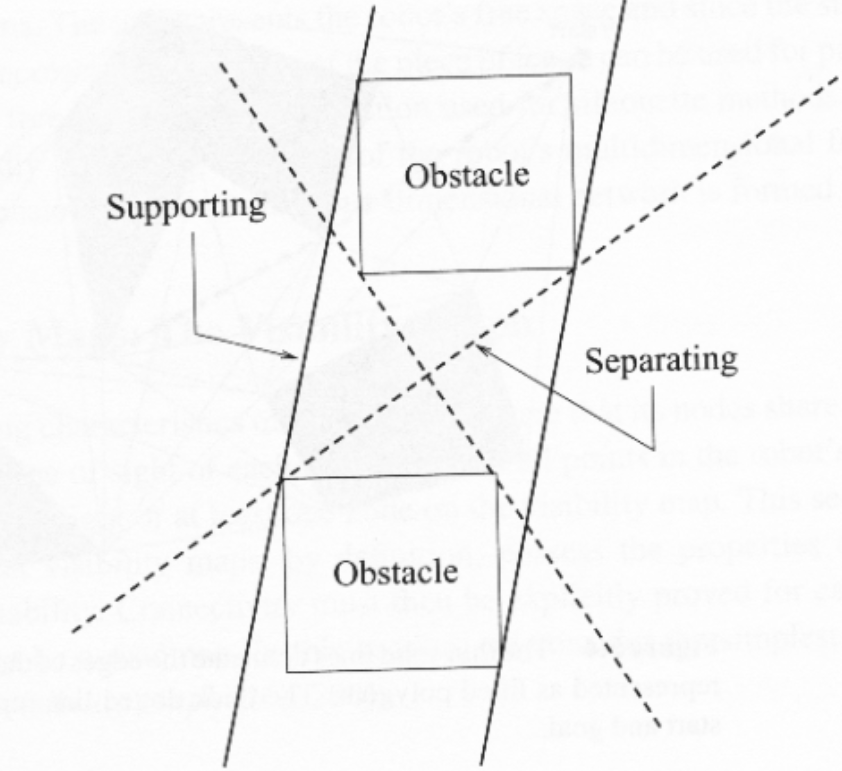
\includegraphics[scale=0.4]{Resources/PNG/SichtGraphReduziert}
		\caption{}
		\label{fig:PNG/SichtGraphReduziert.PNG}
	\end{center}
\end{figure}
\paragraph{Konstruktion des Graphen}
\begin{itemize}
	\item Alle Liniensegmente $vv_i$ mit $v != v_i$ müssen getestet werden, ob sie keinen Schnittpunkt mit einer Kante eines Hindernisses haben
	\item \textbf{Nachteil}: Komplexität O($n^3$)
	\item \textbf{Effizienter}: Plane Sweep Algorithmus mit Komplexität O($n^2 log n$)
\end{itemize}
\newpage
\paragraph{Algorithmus}
\begin{itemize}
	\item \textbf{Input}: A  set of vertices ${v_i}$ (whose edges do not intersect) and a vertex $v$
	\item \textbf{Output}: A subset of vertices from ${v_i}$ that are within line of sight of $v$
\end{itemize}

\begin{itemize}
	\item For each vertex $v_i$, calculate $\alpha$, the angle from the horizontal axis to the line segment $\overline{vv_i}$
	\item Create the vertex list $\epsilon$, containing the $\alpha_i$'s sorted in increasing order.
	\item Create the active list $\mathcal{S}$, containing the sorted list of edges that intersect the horizontal half-line emanating from v.
	\item \textbf{For all} $\alpha_i$ \textbf{do}
	\subitem if $v_i$ is visible to $v$ \textbf{then}
	\subsubitem Add the edge ($v, v_i$) to the visibility graph.
	\subitem \textbf{end if}
	\subitem \textbf{if} $v_i$ is the beginning of an edge, E, not in $\mathcal{S}$ \textbf{then}
	\subsubitem Insert the \textit{E} into $\mathcal{S}$
	\subitem \textbf{end if}
	\subitem \textbf{if} $v_i$ is the end of an edge in $\mathcal{S}$ \textbf{then}
	\subsubitem Delete the edge from $\mathcal{S}$
	\subitem \textbf{end if}
	\item \textbf{end for}
\end{itemize}
\subsection{Voronoi-Diagramme}
\paragraph{Allgemeines Voroni-Diagramm}
\begin{itemize}
	\item Eine Fläche wird willkürlich mit Punkten besetzt $\Rightarrow$ erzeugt Polygonflächen
	\item Alle punkte einer Polygonfläche liegen am nähesten zu dem Punkt der im Zentrum dieses Polygons liegt
	\item Jede Zelle hat genau ein Zentrum
	\item Die Punkte des Gebiets, die zu mehereren Zentren den gleichen Abstand haben, bilden die Grenze zwischen den einzelnen Zellen
	\item Als abstandsfunktion wird der Euklidische Abstand verwendet:
	\subitem $dist(p,q) ) = \sqrt{(p_x-q_x)^2 + (p_y-q_y)^2}$
	\item Das Voronoi-Diagramm ist die Menge solcher Grenzlinien
\end{itemize}
\begin{figure}[H]
	\begin{center}
		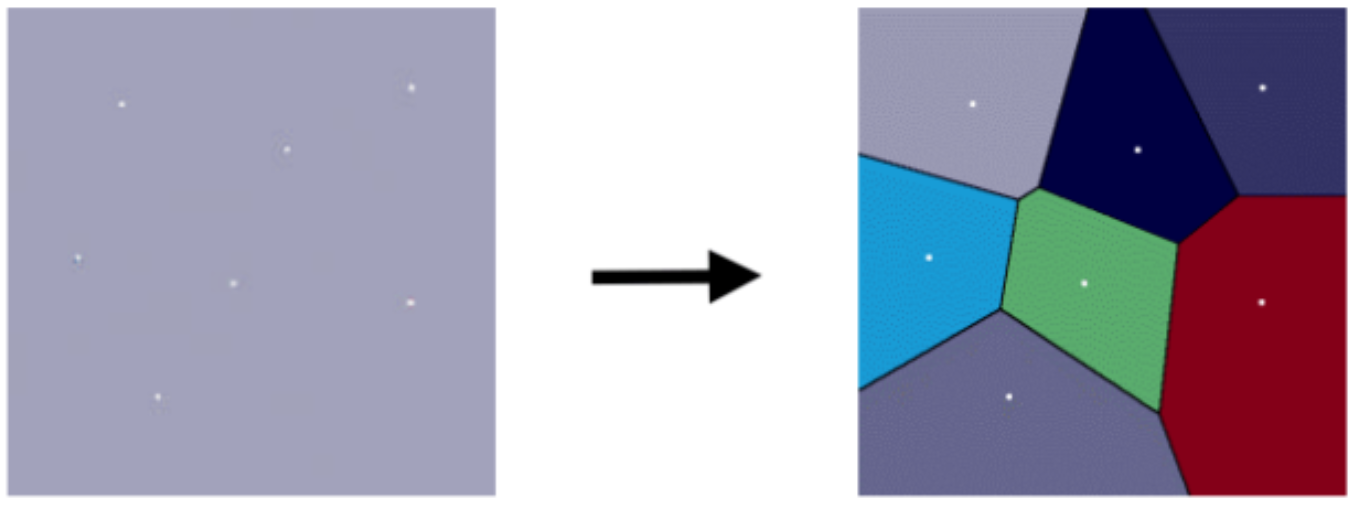
\includegraphics[scale=0.4]{Resources/PNG/Polygon.PNG}
		\caption{}
		\label{fig:PNG/Polygon.PNG}
	\end{center}
\end{figure}
Immer dann gut einsetzbar, wenn ungenaue Sensoren zur Verfügung stehen oder die Umwelt ungenau geometrisch modelliert wurde oder sich dynamisch ändert.
\paragraph{Generalisierte Voronoi-Diagramme}
\begin{itemize}
	\item Bei der Navigation von Robotern wird eine verallgemeinerte Version des Voronoi Diagramms verwendet, das sogenannte \textbf{generalisierte Voronoi Diagramm}(GVD)
	\item \textbf{Generalisierung} betrifft die \textbf{Form der Zentren} und die Art der \textbf{Abstandsfunktion}
	\item \textbf{Zentren} können aus \textbf{komplexeren Formen} wie Linien, Kurven oder Polygonen \textbf{statt Punkten} bestehen
	\item Objekten der Umgebung werden als \textbf{Voronoi-Zentren} behandelt
	\item Die Menge aller \textbf{Voronoi-Kanten}, das GVD, stellt mögliche \textbf{kollisionsfreie Wegstücke} dar
	\item Falls sich der Roboter entlang einer \textbf{Voronoi-Kante} bewegt, kann er nicht mit Hindernissen kollidieren
	\item Beliebtes Verfahren zur Repräsentation des Konfigurationsraumes und Erzeugung eines Graphen.
	\item Punkte an denen sich \textbf{Voronoi-Kanten} schneiden, werden zu \textbf{Voronoi-Knoten}
\end{itemize}
\begin{figure}[H]
	\begin{center}
		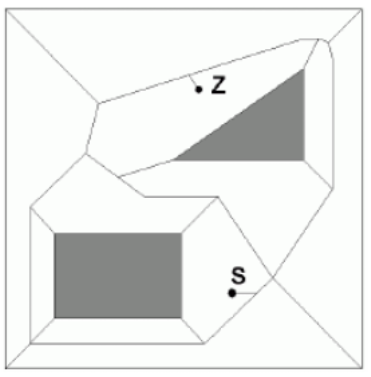
\includegraphics[scale=0.6]{Resources/PNG/Voronoi.PNG}
		\caption{}
		\label{fig:PNG/Voronoi.PNG}
	\end{center}
\end{figure}
Start- und Zielpunkt des gesuchten Weges liegen normalerweise nicht auf dem Diagramm.
Diese beiden Punkte werden mit der nächstliegenden Kante verbunden.
Die Berechnung des optimalen Weges auf dem Voronoi-Diagram kann mit üblichen Graphenalgorithmen vorgenommen werden.
\subsection{Navigation in einer Rasterkarte}
\begin{itemize}
	\item Die Karte ist durch ein binäres Raster mit freiem Platz und Hindernissen gegeben.
	\item Das Raster wird ausgehend vom Startpunkt: \textbf{geflutet} $\Rightarrow$ Füllt den gesamten Hindernisfreien Raum
	\item In jeder Iteration haben alle Pixel auf einer Wellenfront dieselbe Pfadlänge im Raster bezogen auf den Zielpunkt
	\item Backtracking vom Zielpunkt zurück zum Startpunkt und erstellt dabei eine Liste der passierten Rasterpunkte
	\item Gewählt kann jeder Punkt im Raster werden, dessen Wert eins geringer ist, als der aktuell betrachtete
	\item Trifft dies auf mehrere Punkte zu, wird willkürlich einer gewählt
\end{itemize}
\begin{figure}[H]
	\begin{center}
		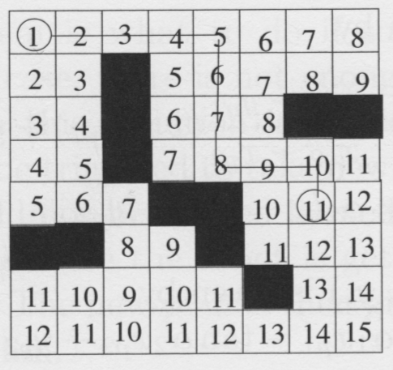
\includegraphics[scale=0.6]{Resources/PNG/RasterKarte.PNG}
		\caption{}
		\label{fig:PNG/RasterKarte.PNG}
	\end{center}
\end{figure}
\paragraph{Fluten der Karte}
\begin{itemize}
	\item Ein \textbf{Rasterpunkt} besitzt vier Nachbarpunkte: \enquote{N}, \enquote{O}, \enquote{S} , \enquote{W}
	\item Ein Rasterpunkt z ist mit 0 für freien Raum belegt und -1 für ein Hindernis
	\item Wenn ein Rasterpunkt eine Nummer erhalten hat, behält er diese Nummer
	\item Der Algorithmus benutzt aus Performancegründen zwei Stacks $S_0$ und $S_1$, die abwechselnd gefüllt und geleert werden. Die Stacks sind anfangs leer
\end{itemize}
\begin{figure}[H]
	\begin{center}
		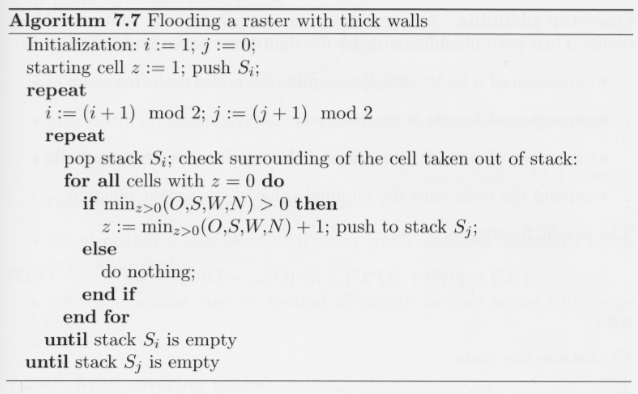
\includegraphics[]{Resources/PNG/Flooding.PNG}
		\caption{}
		\label{fig:PNG/Flooding.PNG}
	\end{center}
\end{figure}
\paragraph{Alternativer Wave Front Planer}
Siehe Ursprungsfolie Kapitel 5, Seite 29/30
\subsection{PotentialFeldmethode}
\paragraph{Grundidee}
\begin{itemize}
	\item Vorbild: \textbf{Elektrisches Feld}
	\item Start- und Zielpositionen, die Positionen aller Hindernisse müssen bekannt sein.
	\item Der \textbf{Zielpunkt und Freiräume} erhalten ein \textbf{anziehendes Potential}
	\item Der \textbf{Startpunkt, die Hindernisse} und Wände erhalten ein \textbf{abstoßendes Potential}
	\item Es wird eine Karte generiert mit virtuell anziehenden und abstoßenden Kräften
	\item Kräfte nehmen linear mit dem Abstand zu den Objekten ab.
	\item \textbf{Ein Objekt bewegt sich nach der Methode des steilsten Abstiegs im Potentialfeld auf das Ziel zu.}
\end{itemize}
\begin{figure}[H]
	\begin{center}
		\includegraphics[scale=0.5]{Resources/PNG/Potentialfeld.PNG}
		\caption{}
		\label{fig:PNG/Potentialfeld.PNG}
	\end{center}
\end{figure}
\chapter{Probabilistische Methoden und Kartierungen}
\section{Problemstellung}
\paragraph{Sensordaten} 
Roboter empfängt regelmäßig Sensordaten, jedoch mit Unsicherheit behaftet.
\paragraph{Steuerdaten}
Roboter führt regelmäßig Bewegungen mit Steuerdaten $u_k$ durch, aber entsprechen nicht exakt den vorgegebenen Steuerdaten.
\paragraph{Position und Umgebungsmodell}
Position schätzt seine globale Position aufgrund der Sensor- und Steuerdaten in seiner Umgebungskarte, jedoch auch mit Unsicherheit behaftet
\section{Modellierung von Unsicherheit}
\begin{itemize}
	\item Viele Aussagen bei mobilen Robotern sind unsicher 
	\item \textbf{Grundlegende Idee} Modellierung von Unsicherheiten durch Wahrscheinlichkeiten
	\item Interpretierung der eigentlichen Lokalisierung als Wahrscheinlichkeitsdichte-Problem
	\item Auch bei weniger präzisen Umgebungsmodellen einsetzbar
	\item Sie erlauben es, den Zustand eines \textbf{dynamischen Systems} probabilistisch zu schätzen
\end{itemize}
\section{Umgebungsmodellierung mit Occupancy Grids}
\subsection{Satz von Bayes}
$p (A|B) = p(B|A) * p(A) / p(B)$
\begin{itemize}
	\item $p(A)$ ist Wahrscheinlichkeit das die Aussage A zutrifft.
	\item $p(A|B)$ bezeichnet die Wahrscheinlichkeit $p(A)$ unter Voraussetzung dass B gilt
\end{itemize}
\subsection{Evidence Grids}
\begin{itemize}
	\item \textbf{Problem}: reale Sensordaten erhalten häufig Rauschen; Rauschen bei Sensordaten führt zu Abweichungen des Idealwerts $\Rightarrow$ schwerwiegende Fehler
	\item Umgebung wird in eine zweidimensionalen Gitternetz repräsentiert
	\item \textbf{Occupancy Grids (Belegungsraster)} speichern in jeder Zelle, ob der Weg für einen Roboter frei oder blockiert ist (\textbf{Binär})
	\item \textbf{Evidence Grids (Beweisraster)} Untermenge der Occupancy Grids. Sammeln Beweismaterial und erstellen damit Karten (\textbf{Belegte Zellen nach Satz von Bayes})
	\item Anhand von Sensordaten wird die Umgebung in einzelne Kartenzellen zergliedert, denen jeweil eine Besetzwahrscheinlichkeit der näheren Umgebung zugewiesen wird.
\end{itemize}
\subsection{Anwendung des Satzes von Bayes}
\begin{itemize}
	\item Die Information über das Verhalten des Sensors wird mit einbezogen
\end{itemize}
\[
	z(x,y)= \frac{p(Zelle belegt \ | \ Sensorwert)}{p(Zelle \ nicht \ belegt \ | \ Sensorwert)}
\]
\begin{itemize}
	\item Die Anwendung des Satzes von Bayes auf diese Formel führt letztlich zu:
\end{itemize}
\[
	z(x,y) = \frac{p(Sensorwert \ | \ Zelle  \ belegt) * p(Zelle \ belegt)}{p(Sensorwert \ | \ Zelle \ nicht \ belegt) * p(Zelle \ nicht \ belegt}
\]
\begin{itemize}
	\item Die Wahrscheinlichkeit, dass eine Zelle belegt ist oder nicht belegt ist, wird zu Beginn mit 0.5 angenommen
	\item Dieser Wert wird fortlaufend mittels der aktuellen Sensorwerte aktualisiert.
	\item Die direkte Anwendung des Bayessischen Filters auf das Selbstlokalisierungsproblem ergibt sich die sogenannte Markov-Lokalisierung
\end{itemize}
\section{Bayes-Filter Algorithmus}
\subsection{Algorithmus}
\begin{itemize}
	\item Vertrauenszustand (\textbf{belief}) spiegelt interne Wissen des Roboters über den Zustand seiner Umgebung wider
	\item Rekursiver Algorithmus: $bel(x_t)$ zum Zeitpunkt $t$ wird berechnet aus dem belief bel($x_t-1$) zum Zeitpunkt $t-1$
	\item $z_t$: letzte Information über den momentanen Umgebungszustand mittels Sensoren (\textbf{Observationsmesswert})
	\item $u_t$ letzte Kontrolldaten, Zustandsänderung im Zeitintervall ($t-1$; $t$) (\textbf{Aktionsmesswert})
	\item $x_t$ Zuszand zum Zeitpunkt $t$
	\item bei $(x_t) = p(x_t |z_1:t, u_1:t)$ ist die \textbf{Wahrscheinlichkeitsverteilung} über den \textbf{Zustand $x_t$ zum Zeitpunkt $t$}, abhängig von allen vergangenen Sensorinformationen $Z_1:t$ und Kontrolldaten $u_1:t$ 
\end{itemize}
%Funktionsweise Siehe Seite 6-8
\section{Markov Lokalisierung}
\subsection{Algorithmus}
\begin{itemize}
	\item Anwendung des Bayes-Filter auf das Lokalisierungsproblem erfordert eine \textbf{Karte als Input}
	\item Probabilistische Verfahren bedienen sich zur Schätzung der a posteriori Wahrscheinlichkeit der \textbf{Markov-Annahme} oder Unabhängigkeitsannahme.
	Nachfolgender Zustand hängt nur vom aktuellen Zustand und nicht von der Historie ab.
	\item Ziel der Markov Lokalisierung ist es, jeder möglichen Roboterposition einen Wahrscheinlichkeitswert zuzuordnen.
	\subitem Position völlig unbekannt $\Rightarrow$ Gleichverteilung
	\subitem Position bereits durch Odometrie oder ähnliches eingeschränkt $\Rightarrow$ Verteilung auf eingegrenzten Bereich verteilt
	\subitem Wenn die Position bekannt ist, folgt die Wahrscheinlichkeit für diese Position = 1
\end{itemize}
\begin{itemize}
	\item Markov Lokalisierung benötigt möglichst genaues Umgebungsmodell
\end{itemize}
\begin{figure}[H]
	\begin{center}
		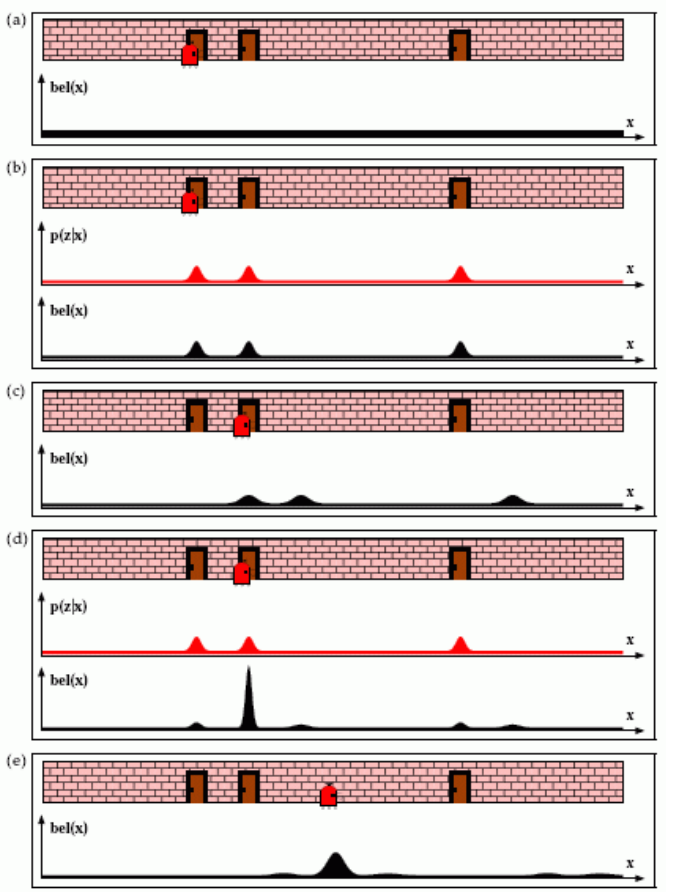
\includegraphics[scale=0.4]{Resources/PNG/MarkovAlgorithmus.PNG}
		\caption{Markov Algorithmus}
		\label{fig:Resources/PNG/MarkovAlgorithmus.PNG}
	\end{center}
\end{figure}
\newpage
\section{Monte Carlo Lokalisierung}
\subsection{Grundsätzliches Vorgehen}
\begin{itemize}
	\item Stichprobenbasierendes Approximationsverfahren
	\item Spezialform von Markov Lokalisierung
\end{itemize}
\begin{figure}[H]
	\begin{center}
		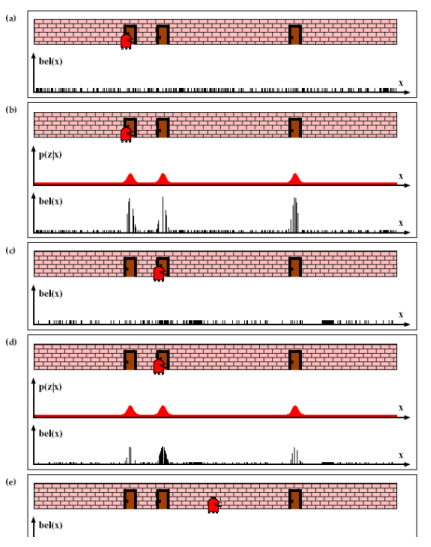
\includegraphics[scale=0.6]{Resources/PNG/MonteCarlo.PNG}
		\caption{Monte Carlo Lokalisierung}
		\label{fig:PNG/MonteCarlo.PNG}
	\end{center}
\end{figure}
\paragraph{Definition}
\begin{itemize}
	\item iterativer Bayesscher Filter, welcher als Schätzer für die zukünftige Wahrscheinlichkeitsverteilung der Roboterposition verwendet wird
	\item Unterscheidet sich im Gegensatz zu gridbasierten Lokalisierungsverfahren in der Betrachtung und in der Verarbeitung
	\subitem \textbf{Praxis}: viele der Gitterzellen besitzen Wahrscheinlichkeit von 0
	\subitem Miteinbeziehung dieser Gitterzellen in Berechnungen $\Rightarrow$ ineffizient
	\subitem diese können vernachlässigt werden
	\subitem fokusieren der Gitterzellen, die die wahrscheinlichsten Positionen widerspiegeln
\end{itemize}
\paragraph{Funktionsweise}
\begin{itemize}
	\item Positionsschätzung bei $(x_k)$ wird durch eine Menge von \textbf{Partikeln} dargestellt
	\item Es besteht keine Information über die Anfangsposition; Partikel sind \textbf{zufällig verteilt}
	\item Durch \textbf{Sensormessung $z$} werden die \textbf{Gewichte} (Strichhöhe) verändert
	\item \textbf{Resampling}: Aus der Partikelmenge werden zufällig aber entsprechend ihrem Gewicht Partikel gezogen $\Rightarrow$ integrierung des Steuerbefehls $(u_k)$ integriert.
	\item Es erfolgt eine erneute Gewichtung mit einem neuen Sensorwert
	\item Anschließend ein erneuetes Resamplung und Integrierung des Steuerbefehls
\end{itemize}
\paragraph{Vorteil}
\begin{itemize}
	\item zur Laufzeit kann die Größe der Stichprobenmenge variabel sein
	\item je unsicherer die Roboterposition ist, desto größer ist die Stichprobenmenge
\end{itemize}
\subsection{Partikelmengen}
\begin{itemize}
	\item Jeder Partikel stellt eine \textbf{Hypothese} für den \textbf{Zustand $x$} dar
	\item Generierung einer Partikelmenge X aus einer Wahrscheinlichkeitsichte p:
\end{itemize}
\begin{figure}[H]
	\begin{center}
		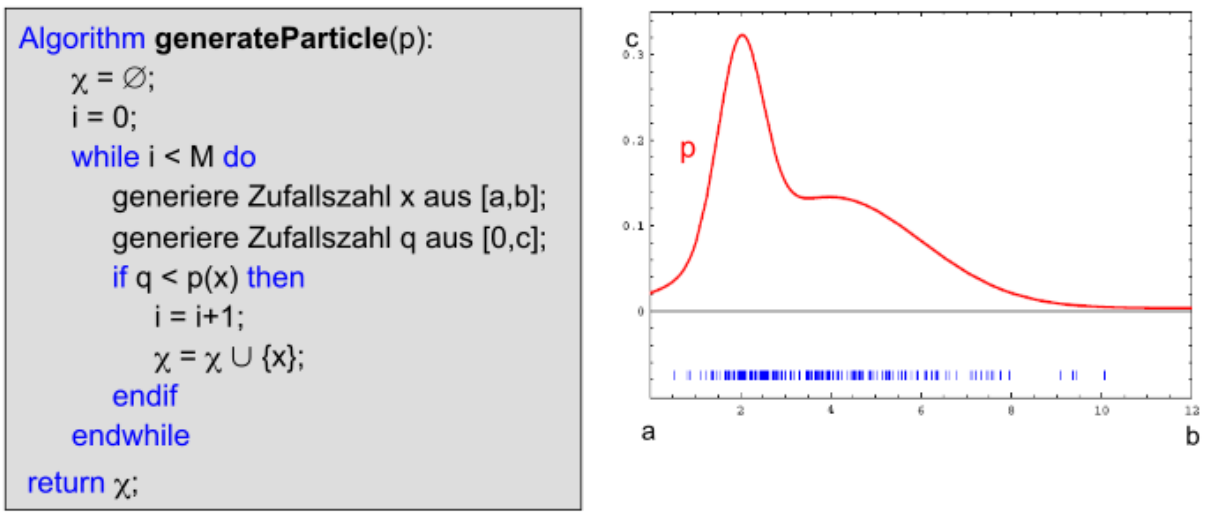
\includegraphics[scale=0.5]{Resources/PNG/PartikelMengen.PNG}
		\caption{Partikelmengen}
		\label{fig:PNG/PartikelMengen.PNG}
	\end{center}
\end{figure}
\section{Kalman-Filter}
\subsection{Definition}
\begin{itemize}
	\item Zustandsschätzer für dynamische Systeme
	\item Spezielle Version eines Bayes-Filters
	\item Dient zur Fusion von zwei unterschiedlichen, stochastisch unabhängigen Informationsquellen
\end{itemize}
\paragraph{Anwendung} fusion der Odometriedaten mit externen Messungen
\subsection{Vorgehen}
\begin{itemize}
	\item $Bel(x_t)$ wird durch seinen Erwartungswert $\mu$ sowie die Kovarianz $\sum_t$ approximiert.
	\item Zu jedem Zeitpunkt wird eine \textbf{Zustandsschätzung} geliefert, die aus einer Schätzung des aktuellen Zustandes und aus einer Vorhersage des Nachfolgezustandes nach Ausführung einer Aktion besteht.
	\item In die \textbf{Zustandsschätzungen} werden unabhängige Sensormessungen integriert
	\item In der \textbf{Vorhersagephase} benutzt der Kalman Filter die Zustandsschätzung vom vorhergehenden Zeitschritt um Zustandsschätzung für den aktuellen Zeitschritt zu erzeugen
	\item In der \textbf{Update} oder \textbf{Korrekturphase} werden die Messinformationen des aktuellen Zeitschritts verwendet, um die Vorhersage zu verbessern.
	\item Das Fehler Modell der Schätzung soll optimal aktualisiert werden auf Basis vorhandener Informationen
\end{itemize}
\subsection{Einschränkungen}
\begin{itemize}
	\item Fehlermodelle sind Gaußverteilungen
	\item Die Zustandsverteilung ist eine Gaußverteilung
\end{itemize}
\begin{figure}[H]
	\begin{center}
		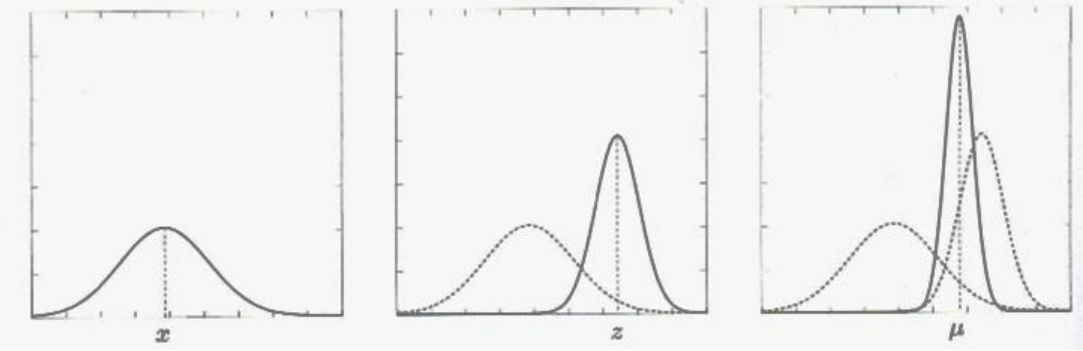
\includegraphics[scale=0.4]{Resources/PNG/KalmanFilter.PNG}
		\caption{Kalman Filter}
		\label{fig:PNG/KalmanFilter.PNG}
	\end{center}
\end{figure}
\begin{itemize}
	\item \textbf{Links}: Unsicherheit im aktuellen Zustand x
	\item \textbf{Mitte}: eine unabhängige Messung z liefert konkurrierende Informationen (\textit{Mittelwewrt und Varianz})
	\item \textbf{Rechts:} Fusion beider Daten liefert eine Mittelung, gewichtet mit der Sicherheit der Informationen, sowie reduzierte Varianz, d.h. eine größere Sicherheit in dem gefilterten Zustand
\end{itemize}
\section{Simultaneous Localization and Mapping}
\subsection{Landmarkenbasiertes SLAM Problem}
\paragraph{SLAM} Simultaneous Localization and Mapping
\begin{itemize}
	\item \textbf{Ausgangspunkt} Roboter exploriert eine unbekannte, statistische Umgebung
	\subitem Roboter kennt seine Pose (Position und Orientierung) nicht genau
	\subitem Es existiert keine Karte der Umgebung
	\item \textbf{Bekannt} sind Sensor- und Steuerdaten: $d = u_1, z_1, u_2, z_2 ... u_k, z_k$
	\item \textbf{Gesucht} Karte $m$ mit $M$ Landmarken: $m = l_1, x, l_1, y, ..., l_M,x,l_M,y$
	\item Weg des Roboters $x_1, x_2, ... x_k$
\end{itemize}
\paragraph{Probablisistische Algorithmen}
\begin{itemize}
	\item Ungenauigkeiten in den Messdaten werden durch Wahrscheinlichkeitsverteilungen modelliert
	\subitem bekannt sind die \textbf{Roboter Bewegungsbefehle} (die Kontrolldaten, die Steuerkommandos $u_t$)
	\subitem bekannt sind die \textbf{Beobachtungen} $z_t$ der nahe gelegnen \textbf{Landmarken} bestehend aus Entfernung und Winkel
	\subitem die Sensorik kann sowohl die Beobachtungsrichtung als auch die beobachtete Entfernung einer Landmarke zur Verfügung stellen
	\subitem gesucht ist eine Schätzung der Karte der Merkmale, der Landmarkenpositionen, sowie der Pfad des Roboters, d.h. seine aktuelle und frühere Posen
\end{itemize}
\subsection{Problemstellung}
\begin{itemize}
	\item Roboterpfad und Positionen der Landmarken in der Karte sind unbekannt
	\item Die Zuodnung von Messdaten zu Landmarken sind i.d. Regel unbekannt
	\item Roboter muss entscheiden, ob Messdaten einer bereits beobachteten Landmarke zugeordnet werden können oder einer noch nicht gesehenen Landmarke
	\item Problematik der Zuordnung wird durch Unsicherheit in der Roboterposition verstärkt
\end{itemize}
\begin{figure}[H]
	\begin{center}
		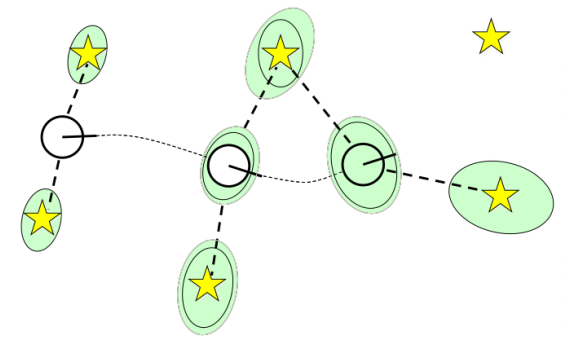
\includegraphics[scale=0.5]{Resources/PNG/ProbabilisitischeLandmarken.PNG}
		\caption{}
		\label{fig:PNG/ProbabilistischeLandmarken.PNG}
	\end{center}
\end{figure}
\subsection{Funktionsweise}
\begin{figure}[H]
	\begin{center}
		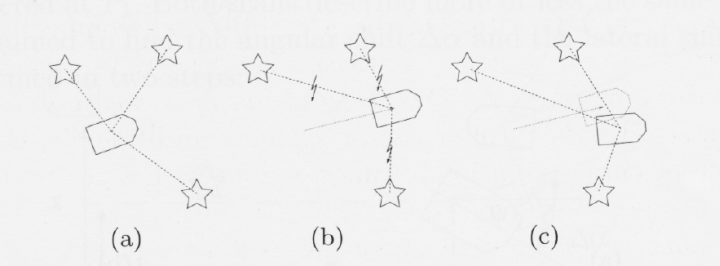
\includegraphics[scale=0.5]{Resources/PNG/FunktionsweiseSLAM.png}
		\caption{SLAM Darstellung}
		\label{fig:PNG/FunktionsweiseSLAM.png}
	\end{center}
\end{figure}
\begin{itemize}
	\item \textbf{(a)} Roboter misst Distanzen zu den Landmarken
	\item \textbf{(b)} Roboter schätzt seine neue Position anhand von Odometriedaten; Odometrie-basierte Roboterpose kann zur Schätzung der neuen Distanzen zu den in \textbf{(a)} verwendeten Landmarken herangezogen werden
	\item Nach Vergleich zwischen Roboter und Landmarken kann der Roboter seine Position \textbf{(c)} korrigieren
\end{itemize}
\subsection{Hinzunahme neuer Landmarken}
\begin{figure}[H]
	\begin{center}
		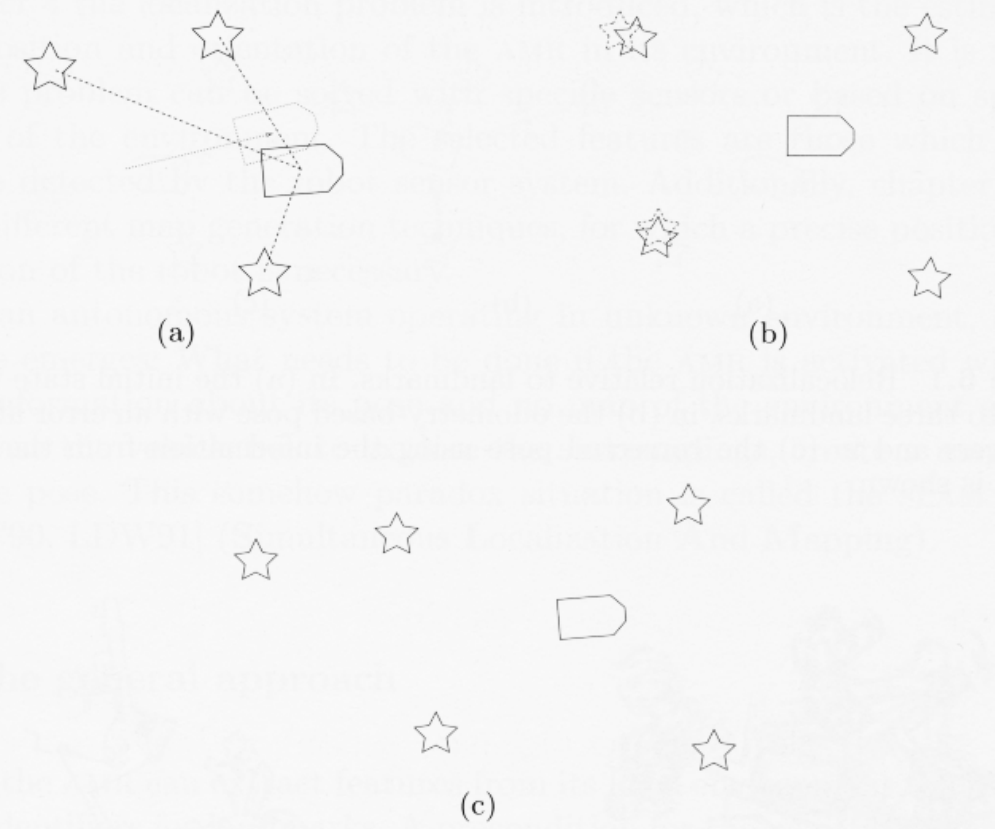
\includegraphics[scale=0.5]{Resources/PNG/LandmarkenErweitern.PNG}
		\caption{}
		\label{fig:PNG/LandmarkenErweitern.PNG}
	\end{center}
\end{figure}
\begin{itemize}
	\item (a) entspricht der Situation aus der vorhergehenden Folie.
	\item In (b) lokalisiert sich das Fahrzeug nach einer Bewegung erneut anhand zweier \enquote{alter} Landmarken und der letzten lokalen Karte
	\item Führt aufgrund der Fehler zu einer ungenauen, globalen Roboterposition
	\item Die Position der neuen Landmarken wird relativ zu der vermeintlich bekannten, korrekten Position der alten Landmarken bestimmt
	\item Positionsannahme ist inkorrekt
	\item Verschiebung der Position der \enquote{alten} Landmarken wird geschätzt und korrigiert sowie auf die Position der neuen Landmarken angewandt
\end{itemize}
\subsection{Aufbau eines SLAM-Graphen}
\begin{itemize}
	\item Sämtliche Messvorgänge sind fehlerbehaftet, auch die Positionsbestimmung der Landmarken
	\item Die Unsicherheit wird in der folgenden Abbildung als Fehlerellipse dargestellt.
	\item Roboter schätzt die Landmarken \textbf{A} und \textbf{B}
	\item nach Bewegung des Roboters nimmt die Genauigkeit der Lokalisierung ab
	\item Die Unsicherheit der Positionsschätzung der Landmarken \textbf{C} und \textbf{D} steigt
	\item Der Roboter erkennt eine bereits zuvor gesehene Landmarke
	\item Eine Verknüpfung mit der früheren Information über die Landmarke reduziert die Unsicherheit bei der Positionsbestimmung und damit auch die Unsicherheit über die zugehörigen früheren Roboterpositionen
\end{itemize}
\begin{minipage}[]{0.5\textwidth}
\begin{figure}[H]
	\begin{center}
		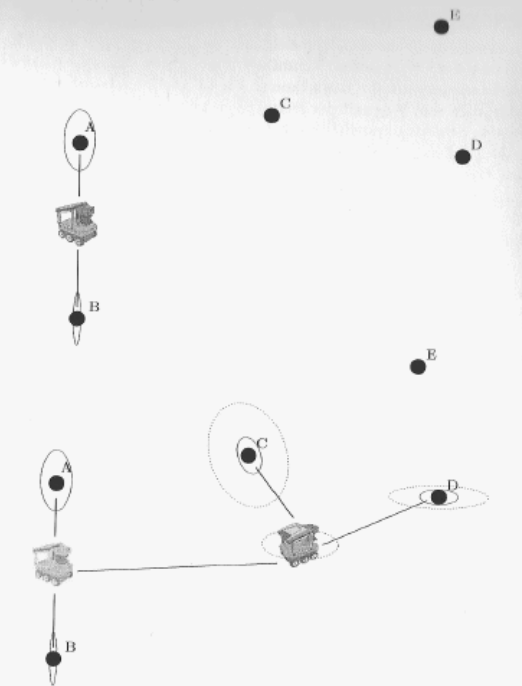
\includegraphics[scale=0.52]{Resources/PNG/LandmarkenBeispiel.PNG}
		\caption{}
		\label{fig:PNG/LandmarkenBeispiel.PNG}
	\end{center}
\end{figure}
\end{minipage}
\begin{minipage}[]{0.5\textwidth}
\begin{figure}[H]
	\begin{center}
		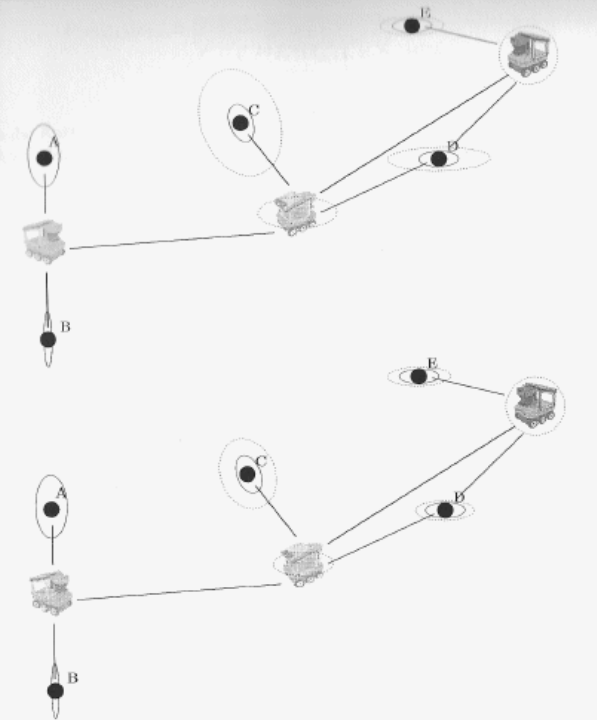
\includegraphics[scale=0.5]{Resources/PNG/LandmarkenBeispiel2.PNG}
		\caption{}
		\label{fig:PNG/LandmarkenBeispie2l.PNG}
	\end{center}
\end{figure}
\end{minipage}
\subsection{Varianten von SLAM}
\paragraph{Vollständiges SLAM}
\begin{itemize}
	\item Roboter schätzt eine Umgebungskarte $m$
	\item Roboter schätzt seine aktuelle Pose $x_t$ und \textbf{alle} zurückliegenden Posen $x_t-1$ bis $x_1$
	\item Grundlage sind die bisher wahrgenommenen Sensordaten $z_1:t$
	\item Sowie alle ausgeführten Aktionen $u_1:t-1$
	\item Es muss die Verteilung $P(m, x1:t | z_1:t, u1:t-1)$
\end{itemize}
\paragraph{Inkrementelles Slam}
\begin{itemize}
	\item Roboter schätzt nur die Karte $m$ sowie die aktuelle Position $x_t$
	\item Es muss die Verteilung $P(m, x_t | z1:t, u1:t-1)$ geschätzt werden
\end{itemize}
\subsection{Bayesian Netzwerk für landmarkenbasiertes SLAM}
\begin{itemize}
	\item Die einzelnen Landmarken sind unabhängig
	\item Gegeben sind die Roboterposen
\end{itemize}
\begin{figure}[H]
	\begin{center}
		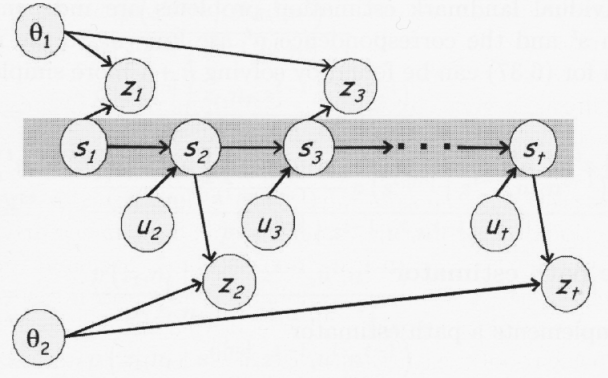
\includegraphics[scale=0.8]{Resources/PNG/BayesNetzwerk}
		\caption{Bayes Netzwerk}
		\label{fig:PNG/BayesNetzwerk}
	\end{center}
\end{figure}
Modell von Variablen und deren Abhängigkeiten als dynamisches Bayes-Netzwerk.
\begin{itemize}
	\item Kern des Modells bilden die
	\subitem Zeitreihe der Roboterzustände $s_1, s_2, ... s_t$
	\subitem die Positionen der Landmarken $\theta_k$
	\subitem die Kontrollvariablen $u_t$
	\subitem und die gemessenen, beobachteten Landmarken Positionen $z_t$
	\item Der Roboter bewegt sich von $s_1$ nach $s_t$ mit einer Folge Kontrolleingaben $u_2, ... u_t$
	\item Der Roboterzustand $s_t$ zum Zeitpunkt $t$ ist lediglich vom Roboterzustand $s_t-1$ zum vorhergehenden Zeitpunkt und dem ausgeführten Steuerkommando $u_t$ des Roboters abhängig
	\item Zum Zeitpunkt $t = 1$ beobachtet der Roboter die Landmarkenpositionen $\theta_1$ mittels $z_1$ zum Zeitpunkt $t = 2$ beobachtet er $\theta_2$ via $z_2$ und zum Zeitpunkt $t = 3$ wieder $\theta_1$
	\item Die Beobachtung $z_t$ ist abhängig von der globalen Position der Landmarke $\theta_k$ und dem aktuellen Roboterzustand $s_t$
	\item \textbf{FastSLAM} zerlegt das Problem
	\subitem in die \textbf{Lokalisation} (Wissen über den vom Roboter zurückgelegten weg  $s_1, ... s_t$)
	\subitem und einer Sammlung von einzelnen \textbf{Landmarken-schätzungen} $z_k$, die von der geschätzter Roboterpose abhängen
	\item Zeitkomplexität von \textbf{FastSLAM} ist $O(f M)$
	\subitem $f$ konstanter Faktor
	\subitem $M$ Anzahl der Landmarken
\end{itemize}






















\chapter{Schwarmrobotik und Evolutionäre Robotik}
\section{Schwärme  und deren Verhalten in der Natur}
\paragraph{Schwarmdefinition}
Der Begriff \textbf{Schwarm} bezeichnet einen Verband von fliegenden oder schwimmenden Lebewesen, der sich koordiniert bewegt.
Im Unterschied zu anderen Gruppen zeigt er ein sogenanntens \textbf{Schwarmverhalten}
\subsection{Computersimulation von Schwärmen - Algorithmus von Craig Reynolds}
Die einzelnen Individuen agieren in Abhängigkeit von der Position und der Geschwindigkeit der benachbarten Boids nach folgenden Regeln:
\paragraph{Separation} Bewege dich weg sobald dir andere zu nahe kommen
\paragraph{Alignment} Bewege dich in die gleiche Richtung wie deine Nachbarn
\paragraph{Cohesion} Bewege dich zum Mittelpunkt der benachbarten Vögel
\paragraph{Vorraussetzung}
Reynolds setzte vorraus, dass \textbf{alle} Vögel innerhalb eines fixen gegebenen Radius interagieren.
Die Nachbarschaft ist bei Reynolds charakterisiert durch einen Abstand vom Zentrum des Vogels und durch einen bestimmten Winkel ausgehend von der Flugrichtung.
Tiere außerhalb dieser Nachbarschaft werden ignoriert.
\section{Schwarmintelligenz}
Unter \textbf{Schwarmintelligenz} versteht man Systeme bestehend aus vielen primitiven, mobilen Agenten, die:
\begin{itemize}
	\item gemeinsam agieren
	\item miteinander kommunizieren können
	\item im Kollektiv ein komplexes Problem lösen
	\item ohne zentrale Steuerung sich selbst organisieren
\end{itemize}
\paragraph{Kollektive Intelligenz} Die Individuen agieren ziemlich beschränkt, die Gesellschaften dagegen sind ungemein leistungsfähig.
Geeignet zur \textbf{Lösung schwieriger Optimisierungsprobleme}
\section{Multi Robot Systems}
Einsatz von simplen Robotern, deren Handlungsmöglichkeiten und Wahrnehmungssysteme stark begrenzt sind.
\paragraph{Vorteile}
\begin{itemize}
	\item \textbf{robust}
	\item \textbf{skalierbar}
	\item \textbf{flexibel}
	\item \textbf{Kosten} statt eines euren einzelnen Roboters, der eventuell nicht so leicht oder schnell zu ersetzen ist, werden billige Komponenten eingesetzt.
	\item \textbf{Verlässlichkeit} wenn ein einzelner Roboter oder Softwareagent ausfällt übernehmen andere Roboter dessen Aufgabe und fügen sich neu ins Kollektiv
	\item \textbf{Flexibilität} viele kleine kooperierende Roboter können bei sinnvoller Zusammenarbeit Probleme bewältigen, die ein großer Roboter alleine eventuell nicht bewältigen kann.
\end{itemize}
\paragraph{Problem} Das Schwarmverhalten ist aufgrund des Einzelverhaltens nur schwer vorhersagbar.
\section{Ameisenalgorithmen}
\subsection{Optimaler Weg bei futtersbeschaffenden Ameisen}
\paragraph{Funktionsweise}
\begin{itemize}
	\item Eine Ameise verlässt den Bau, das nest (N) und sucht Futter auf einem \textbf{zufälligen Weg}
	\item Es gibt mehrere Zweige zur Futterquelle
	\item Weg wird mit \textbf{Pheromon}, einer chemischen Substanz markiert.
	\item Findet die Ameise Futter, schleppt sie das Futter auf dem gleichen oder einem anderen Weg zurück, der Weg wird dabei ev. ein weiteres Mal markiert.
	\item Weitere Ameisen, die zur Futtersuche starten, \textbf{orientieren sich} bei der Futtersuche \textbf{an den Pheromonspuren}
	\item Ameisen folgen \textbf{bevorzugt}, aber nicht immer den markierten Wegen
	\item Auf langen Wegen ist die Ameisendichte wegen der größeren Entfernung geringer, das Pheromon verdunstet schneller.
	\item Wenn ein Ausreißer einen kürzeren Weg findet und einige andere Ameisen beginnen diesem Weg zu folgen, wird die Ameisendichte auf dem längerenWeg immer geringer und der kürzere Weg setzt sich durch
\end{itemize}
\begin{figure}[H]
	\begin{center}
		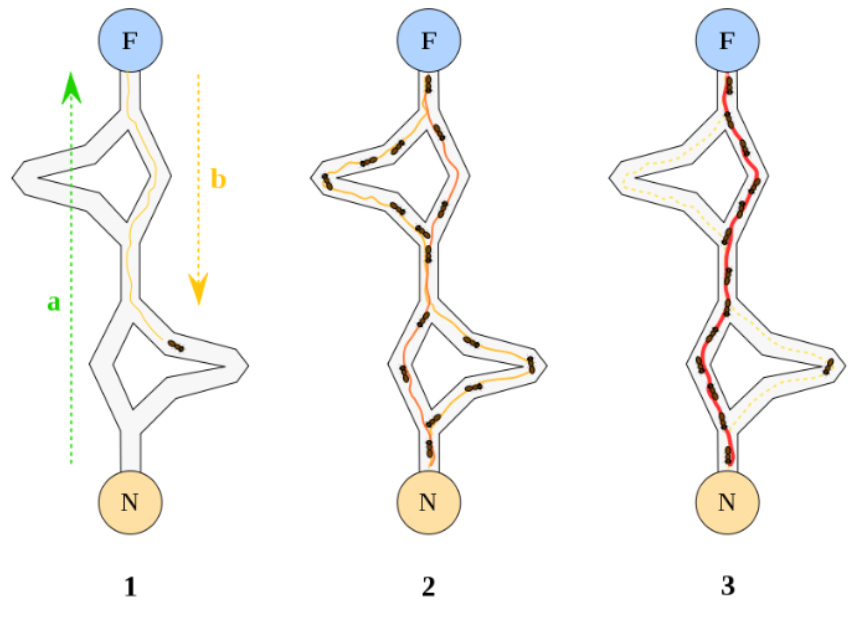
\includegraphics[scale=0.6]{Resources/PNG/AmeisenAlgorithmus.PNG}
		\caption{Darstellung des Ameisenalgorithmus Prinzips}
		\label{fig:PNG/AmeisenAlgorithmus.PNG}
	\end{center}
\end{figure}
\subsection{Ant Colony Optimization Algorithm}
\begin{itemize}
	\item \textbf{Ant Colony Optimization(ACO)} ist der Überbegriff für Ameisen-basierende Algorithmen
\end{itemize}
\paragraph{Kategorien}
\begin{itemize}
	\item \textbf{Tourenplanung (Routing)}: $\Rightarrow$ Travelling Salesman Problem
	\item \textbf{Zuordnung (Assignment)}: optimale Zuordnung von Personen oder Betriebsmitteln auf Stellen oder Aufgaben
	\item \textbf{Ablaufplanung (Scheduling)}: Verteilung von knappen Ressourcen auf Prozesse die zeitlich begrenzt sind
	\item \textbf{Teilmengen Problem (Subset)}: aus einer Menge von Objekten muss eine Teilmenge gefunden werden, damit eine vorgegebene Bedingung erfüllt und eine Zielfunktion optimiert wird. 
\end{itemize}
\paragraph{Eigenschaften}
\begin{itemize}
	\item optimaler Weg ist der \textbf{kürzeste Weg} zwischen zwei Punkten
	\item \textbf{globale Information}: Belegung mit künstlichen Pheromonen als zentrale Idee
	\item Wahrscheinlichkeits-gestützte, \textbf{lokale Entscheidungen} - Ameise erkennt unmittelbare Nachbarschaft
\end{itemize}
\paragraph{Funktionsweise}
\begin{enumerate}
	\item Ameisen laufen entlang des Graphen
	\item Eine Ameise erzeugt eine Lösung gemäß lokaler Information und Pheromon
	\item Update beinhaltet neu aufgetragene Pheromone und Verdunstung bereits vorhandener Pheromone
	\item Operationen, die globales Wissen vorraussetzen und damit nicht von einzelnen Ameisen bewerkstelligt werden können
\end{enumerate}
\begin{itemize}
	\item Diskretisierung der Zeit t: in einem Zeitschritt erzeugen alle Ameisen eine vollständige Lösung.
	\item Eine \textbf{Pheromon-Matrix} enthält die  Intensität der Pheromone $T_ij(t)$ enthält die Intensität der Pheromone auf einer Kante vom Knoten $i$ zum Knoten $j$ im Graphen
	\item Eine Matrix für lokale Informationen enthält die Sichtbarkeit der Stadt (d.h. die jeweils reziproke Distanz): $n_ij = \dfrac{1 }{d_ij}$
\end{itemize}
\subsection{Traveling Salesman Problem}
\begin{itemize}
	\item Vorhanden: \textbf{vollständiger gerichteter Graph} 
	\item Gesucht: \textbf{Rundtour durch alle Städte}
\end{itemize}
Ameisen laufen durch den Graphen, die Kolonie ermittelt den Optimalen Weg.
\begin{itemize}
	\item Es erweist sich als vorteilhaft, für jede Ameise eine andere zufällig gewählte Stadt als Ausgangspunkt für die Tour zu nehmen
\end{itemize}
\paragraph{Algorithmus - Schritte}
\begin{figure}[H]
	\begin{center}
		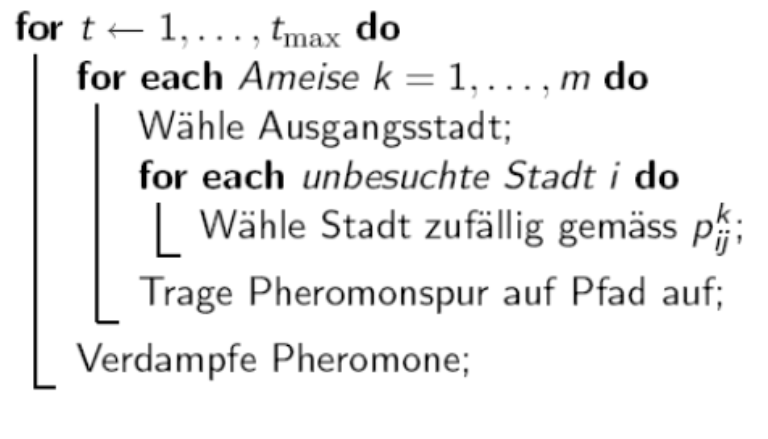
\includegraphics[scale=0.5]{Resources/PNG/ACO.PNG}
		\caption{Ameisenalgorithmus - Schritte}
		\label{fig:PNG/ACO.PNG}
	\end{center}
\end{figure}
\paragraph{Entscheidung für nächste Stadt}
\begin{itemize}
	\item Jede Ameise besitzt eine Liste mit gültiger Nachbarschaft $N$
	\item Die Entscheidung in einem Knoten bzgl. der nächsten Stadt fällt gemäß folgender Formel:
\end{itemize}
$p_{i j}^{k}=\left\{\begin{array}{ll}{\frac{\left[\tau_{i j}(t)\right]^{\alpha} \cdot\left[\eta_{i j}\right]^{\beta}}{\sum_{l \in J_{i}^{k}}\left[\tau_{i l}(t)\right]^{\alpha} \cdot\left[\eta_{i l}\right]^{\beta}}} & {\text { für } j \in J_{i}^{k}} \\ {0} & {\text { für } j \notin J_{i}^{k}}\end{array}\right.$
\begin{itemize}
	\item $\alpha$ und $\beta$ steuern das Verhältnis zwischen Anteil der Pheromone und lokaler Information
	\item für $\alpha$ hat man den klassischen Greedy Ansatz
\end{itemize}



\chapter{Locomotion}
\section{Fortbewegungsarten}
\begin{itemize}
	\item Fortbewegungsarten für Roboter sind of durch die Natur inspiriert.
	\item Roboter mit Beinen benötigen in der Regel mehr Freiheitsgrade und sind mechanisch komplexer als Roboter auf Rädern.
\end{itemize}
\section{Laufroboter}
\subsection{Vorteile von Laufrobotern}
\begin{itemize}
	\item Können auf unregelmäßigen Untergrund laufen
	\item Natürliche Fortbewegung
	\item Keine Umweltveränderung erforderlich
\end{itemize}
\subsection{Nachteile von Laufrobotern}
\begin{itemize}
	\item Komplizierte Mechanik
	\item Anspruchsvolle Steuerungssoftware
	\item Mehrere Freiheitsgrade pro Beins
	\item Vielzahl an Sensoren erforderlich
	\subitem interne Sensoren wie Potentiometer, Inkrementalsensoren, ...
	\subitem externe Sensoren wie Stoßdämpfer, Stereo-Kamera, Infrarot, Ultraschall, ...
\end{itemize}
\subsection{Freiheitsgrade für Roboterbeine}
\begin{itemize}
	\item Um ein Bein bewegen zu können, sind mindestens zwei Freiheitsgrade notwendig
	\item Die meisten Laufroboter haben mehrgliedrige Beine mit mindestens drei Freiheitsgraden pro Bein
\end{itemize}
\begin{figure}[H]
	\begin{center}
		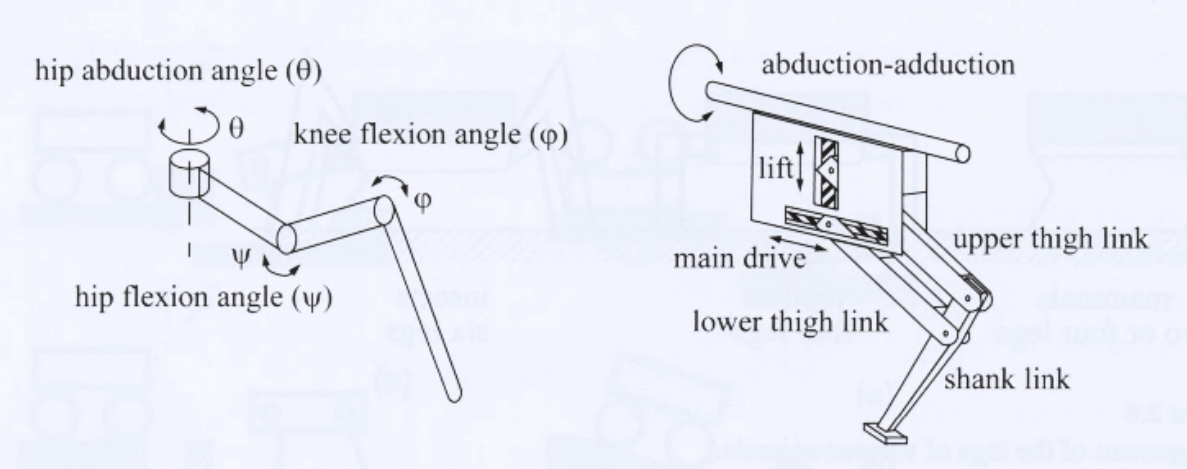
\includegraphics[scale=0.5]{Resources/PNG/RoboterFreiheitsgrade.PNG}
		\caption{Freiheitsgrade für Roboterbeine}
		\label{fig:Resources/PNG/RoboterFreiheitsgrade.PNG}
	\end{center}
\end{figure}
\subsection{Freiheitsgrade für Zweibeiner}
\begin{itemize}
	\item Zweibeiner haben meist sechs Freiheitsgrade pro Bein
	\item Menschliches Bein hat 7 Freiheitsgrade
	\item Die Zahl der unterschiedlichen Gangarten hängt von der Zahl der Beine ab.
	\item Ein Zweibeiner (mit $k=2$) hat $N = (2 \cdot k - 1)! = 6$s unterschiedliche Gangarten
\end{itemize}
\subsection{Laufverhalten}
\begin{itemize}
	\item Das Geh- und Laufverhalten kann in \textbf{statisch und dynamisch stabile Gangarten} eingeteilt werden 
	\item Funktioniert nur für sehr langsame Bewegungen
\end{itemize}
\paragraph{Definition: Statisches stabiles Gehen}
bedeutet, dass sich der Roboter zu jedem Zeitpunkt in einem statischen Körperschwerpunkt ist so über den Füßen, dass der Körper nicht fallen kann.
\paragraph{Definition: Dynamisch stabiles Gehen}
bezeichnet Laufbewegungen, mit weniger als drei Füßen in Kontakt mit dem Boden.
Dynamisches Gehen arbeitet mit Körperschwingungen: der Körperschwerpunkt befindet sich die meiste Zeit außerhalb von der aufgespannten Gleichgewichtszone.
\subsection{Statisch stabiles Gehen}
\begin{itemize}
	\item Statische Stabilitätsbedingung: der Masseschwerpunkt (\textit{Center of Gravity}) ist immer über dem STützpolygon
	\subitem \textbf{Stützpolygon} ist ein minimales Polygon, das alle Kontaktstellen des Roboters mit dem Boden enthält.
	\subitem möglich für alle Beinanzahlen >= zwei
	\subitem nur langsame Bewegungen möglich	
\end{itemize}
\paragraph{Dreifußgang}
\begin{itemize}
	\item Je drei Beine sind in der Stemmphase und in der Schwingphase
	\item Verbindet man die drei Beine in der Stemmphase ergibt sich ein Dreieck
\end{itemize}
\begin{figure}[H]
	\begin{center}
		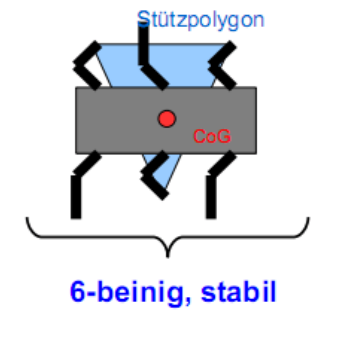
\includegraphics[scale=0.6]{Resources/PNG/DreiBein.PNG}
		\caption{}
		\label{fig:Resources/PNG/DreiBein.PNG}
	\end{center}
\end{figure}
\subsection{Zero Moment Point und Pseudo-Dynamisches Gehen}
\begin{itemize}
	\item Zero Moment Point (ZMP) ist der Punkt auf dem Boden, an dem die Kippmomente null werden
	\item ZMP dominiert seit 40 Jahren das zweibeinige GEhen
	\item Bewährt bei glatten Flächen
	\item Bei zweibeinigen Robotern wird das Stützpolygon ersetzt durch die konvexe Hülle der Bodenkontaktflächen
	\item \textbf{Nachteile des ZMP}
	\subitem ZMP geregelter Gang kann nicht schneller sein als die Sensorik
	\subitem ZMP erfordert die genaue Kenntnis der Massenverteilung im Roboter und alle Gelenkstellungen
\end{itemize}
\subsection{Steuerungssoftware}
\paragraph{Neuronale Netze}
\begin{itemize}
	\item Ähnlich zu biologischen Vorbildern
	\item Training durch Simulation
\end{itemize}
\paragraph{Mechatronik und Regelung}
\begin{itemize}
	\item Regelung von Gelenkwinkel und -Geschwindigkeiten
	\item Trajektorienplanung und -interpolation
	\item Explizite regelbasierte Laufplanung
	\item \textbf{Vorteil:} Nutzung gut bekannter mechatronischer Prinzipien 	
	\item Eigenschaften wie Stabilität sind gut bekannt
	\item Lernen einfacher Steuerungszusammenhänge im Gegensatz zu Neuronalen Netzen nicht notwendig
\end{itemize}
\paragraph{Verhaltensbasierte Steuerungen}
\begin{itemize}
	\item Modellierung von Basisverhalten durch Aufbau von Sensor/Motor-Verbindungen
	\item Zerlegung von komplexem Verhalten zu einer Vielzahl einfacher Ebenen mit zunehmend abstraktem Verhalten
	\item Verhalten können durch ein überlagertes Verhalten beeinflusst werden
	\item Mehrere Basisverhalten können zusammen zu einem völlig neuartigem Verhalten führen
	\item \textbf{Jedoch:} Schwierigkeiten bei der Realisierung komplexer Verhalten.
\end{itemize}
\section{Radroboter}
\subsection{Stabilität von Radrobotern}
\begin{itemize}
	\item Natürliche Bewegungen wie Kriechen, Laufen, Springen oder Gehen technisch schwer zu imitieren.
	\item Mehrheit der mobilen Roboter auf Rädern oder Raupen unterwegs
	\item Alle Räder haben in der Regel Kontakt zum Untergrund
	\item für \textbf{statisch stabile Fahrzeuge} braucht man mindestens drei Räder:
	\subitem Zwei angetriebene Räder auf einer Achse mit einem oder zwei passiv mitlaufenden Stützrädern, die sich frei drehen können
	\subitem Steuerung erfolgt durch verschiedene Geschwindigkeit angetriebener Räder
	\subitem kinematisches Zentrum oft in der Mitte des Fahrzeugs
	\item \textbf{dynamische Stabilität erfordert Bewegung}
\end{itemize}
\section{Kinematik mobiler Radroboter}
\subsection{Holonomische Bewegung}
Eine Bewegung heißt \textbf{holonomisch}, wenn das Objekt seine \textbf{Orientierung und seine Position unabhängig voneinander ändern} kann.
\paragraph{Pose System}
\begin{itemize}
	\item Position eines Objekts auf einer Ebene kann mittels zweier Koordinaten angegeben werden
	\item Die absolute Orientierung des Objektes wird mit einer dritten Koordinate angegeben, was zusammen ein Pose-System ergibt
	\item Koordinaten des Pose Systems $\Rightarrow$ 2 für die Position in x,y Ebene; 1 für die absolute Orientierung
\end{itemize}
\subsection{Kinematik und Positionsveränderung für Zweiradandtrieb}
\begin{itemize}
	\item \textbf{Vorraussetung}: kreisförmiger Roboter mit Zweiradantrieb, Bewegung ist nur in der Ebene möglich
	\item Position: Koordinaten $x,y$, Orientierung $\alpha$
	\item Roboter misst zu diskreten Zeitpunkten $t$ den mit dem linken bzw. mit dem rechten Rad zurückgelegten Weg
	\item $\Delta L$ und $\Delta R$ werden von Radwegsensoren ermittelt
\end{itemize}
\begin{itemize}
	\item Der Drehwinkel $\Delta \alpha$ ist die Wegdifferenz des rechten und des linken Rades geteilt durch den Radabstand $D$ \\
	$\Delta \alpha=\frac{\Delta R-\Delta L}{D}$
	\item Die Wegstrecke ist der mittlere Weg \\
	$\Delta s=\frac{\Delta L+\Delta R}{2}$
	\item Positionsänderung bei Geradeausfahrt mit $\Delta L = \Delta R$ \\
	$\Delta x=\Delta R * \cos (\alpha)$ \\
	$\Delta y=\Delta L * \sin (\alpha)$
\end{itemize}
\subsection{Fortbewegung bei Omnidirektionalem Antrieb}
\begin{figure}[H]
	\begin{center}
		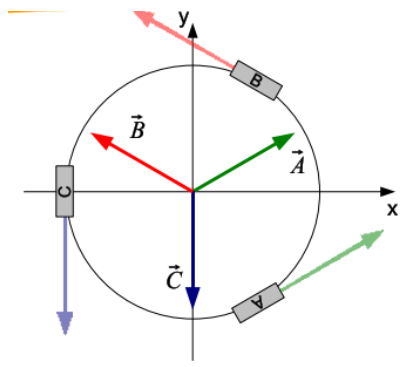
\includegraphics[scale=0.6]{Resources/PNG/EinheitsVektoren.PNG}
		\caption{Einheitsvektoren}
		\label{fig:PNG/EinheitsVektoren.PNG}
	\end{center}
\end{figure}
\begin{itemize}
	\item \textbf{Einheitsvektoren} geben die Richtungen an, in denen die Omniwheels von den drei Motoren angetrieben werden.
	\item \textbf{Geschwindigkeitsvektoren} sind die Einheitsvektoren
	\item Raddrehmomente $\alpha, \beta, \gamma$ proportional zur Winkelgeschwindigkeit des jeweiligen Rades
	\item \textbf{Bewegungsvektor} $\vec{V}=\alpha \cdot \vec{A}+\beta \cdot \vec{B}+\gamma \cdot \vec{C}$
\end{itemize}












	









\chapter{Industrierobotik}
\section{Industrieroboter}
\begin{itemize}
	\item \textbf{Roboterarm} mit Achsen, Gelenken und Antrieben
	\item Steuerung in einem \textbf{Steuerschrank} mit \textbf{Bedienerkonsole}
	\item \textbf{Handsteuergerät}
\end{itemize}
\subsection{Einsatz}
\begin{itemize}
	\item In wohldefinerter Umgebung, definierte Hindernisse, bekannte Umwelt
	\item Größtes Einsatzgebiet in der Automobilindustrie und deren Zulieferern (\textit{Schweißen, Lackieren, Beschichten ...})
\end{itemize}
\subsection{Trends}
\begin{itemize}
	\item Industrie 4.0, KI, IoT
	\item Human-Robot collaboration
	\item Mobile Roboter und einfachere Bedienung
\end{itemize}
\section{Bauform und Komponenten}
\paragraph{Roboterarm}
\begin{itemize}
	\item Armelemente bzw. Glieder die über Bewegungsachsen miteinander verbunden sind.
	\item Ausgleichszylinder $\Rightarrow$ Motoren werden nicht überlastet, geringere Kräfte sind nötig
\end{itemize}
\paragraph{Endeffektor, Hand}
\begin{itemize}
	\item Das Arbeitsorgan $\Rightarrow$ Werkzeug
	\item Üblicherweise wird die Werkzeugspitze \textit{\textbf{Tool Center Point}(TCP)} genannt
\end{itemize}
\paragraph{Fahrzeug}
\begin{itemize}
	\item optional
	\item meist bodengebunden
	\item ein bis drei Freiheitsgrade
	\item Bsp.: Verfahrschlitten
\end{itemize}
\section{Freiheitsgrade}
\subsection{Definition}
Der Freiheitsgrad (DOF) bezeichnet in der Physik die Anzahl der frei wählbaren, voneinander unabhängigen Parameter eines physikalischen Systems, die dessen Zustand eindeutig kennzeichnen.
\begin{itemize}
	\item In der Mechanik drückt der DOF die Möglichkeit aus im Raum voneinander unabhängig Bewegungen auszuführen
	\item Anzahl der Freiheitsgrade drückt die translatorischen und rotatorischen Bewegungsmöglichkeiten eines Körpers aus
	\item Anzahl der Gelenkachsen $\neq$ Anzahl der Freiheitsgrade
\end{itemize}
\section{Bewegungsachsen}
\subsection{Rotatorisch}
\begin{figure}[H]
	\begin{center}
		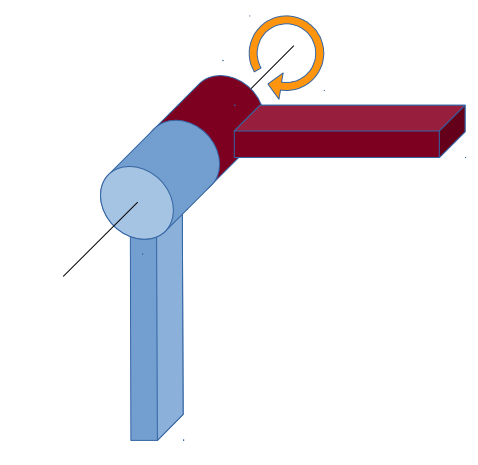
\includegraphics[scale=0.6]{Resources/PNG/Rotatorisch.PNG}
		\caption{Rotatorische Achse}
		\label{fig:PNG/Rotatorisch.PNG}
	\end{center}
\end{figure}
\begin{itemize}
	\item Für Drehbewegungen
	\item Freiheitsgrad: 1
\end{itemize}
\subsection{Translatorisch}
\begin{figure}[H]
	\begin{center}
		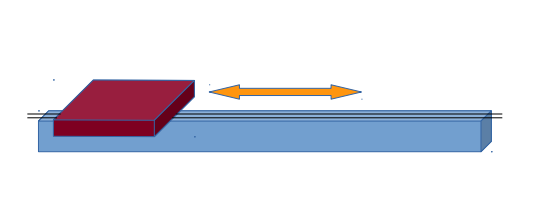
\includegraphics[scale=0.6]{Resources/PNG/Translatorisch.PNG}
		\caption{Translatorische Achse}
		\label{fig:PNG/Translatorisch.PNG}
	\end{center}
\end{figure}
\begin{itemize}
	\item Für Schubbewegungen
	\item Freiheitsgrad: 1
\end{itemize}
\paragraph{Hauptachsen}
\begin{itemize}
	\item Zum Positionieren des Effektors im Raum
	\item Beeinflussen Position des TCP
	\item Rotatorisch oder Translatorisch
\end{itemize}
\paragraph{Nebenachsen}
\begin{itemize}
	\item Kopf- oder Handachsen
	\item Rufen nur kleine Positionsänderungen hervor
	\item Orientierung des Werkzeugs
	\item Meist rotatorisch
\end{itemize}
\subsection{Rotationsgelenk}
Die Drehachse bildet einen rechten Winkel mit den Achsen der beiden angeschlossenen Glieder.
\begin{figure}[H]
	\begin{center}
		
\includegraphics[scale=0.6]{Resources/PNG/Rotationsgelenk.PNG}
		\caption{Rotationsgelenk}
		\label{fig:Resources/PNG/Rotationsgelenk}
	\end{center}
\end{figure}
\subsection{Torsionsgelenk}
Die Drehachse verläuft parallel zu den Achsen der beiden Glieder.
\begin{figure}[H]
	\begin{center}
		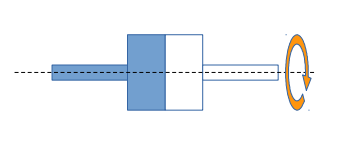
\includegraphics[scale=0.6]{Resources/PNG/Torsionsgelenk.PNG}
		\caption{Torsionsgelenk}
		\label{fig:Resources/PNG/Torsionsgelenk}
	\end{center}
\end{figure}
\subsection{Revolvergelenk}
Das Eingangsglied verläuft parallel zur Drehachse, das Ausgangsglied steht im rechten Winkel zur Drehachse.
\begin{figure}[H]
	\begin{center}
		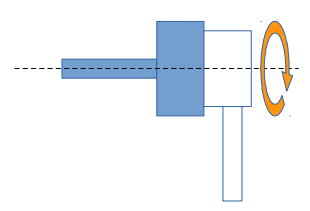
\includegraphics[scale=0.6]{Resources/PNG/Revolvergelenk}
		\caption{Revolvergelenk}
		\label{fig:Resources/PNG/Revolvergelenk}
	\end{center}
\end{figure}
\subsection{Kugelgelenk}
Besitzt 3 Freiheitsgrade, wobei die Beweglichkeit stark eingeschränkt ist.
Arbeitsbereich der X- und Y-Achse wird durch die Konstruktion auf unter 
180 $\deg$ limitiert.
Die Einkerbung an der Vorderseite lässt an dieser stelle einen 90 $\deg$ Winkel zu.
\begin{figure}[H]
	\begin{center}
		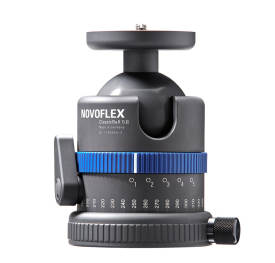
\includegraphics[scale=0.8]{Resources/PNG/Kugelgelenk.PNG}
		\caption{Kugelgelenk}
		\label{fig:Resources/PNG/Kugelgelenk.PNG}
	\end{center}
\end{figure}
\section{Arbeitsraum}
\paragraph{Definition} Punkte im 3D-Raum, die von der Roboterhand angefahren werden können.
\section{Grundtypen von Industrierobotern}
\subsection{Portalroboter}
\begin{itemize}
	\item Steife Struktur $\Rightarrow$ sehr große Arbeitsräume möglich
	\item Sehr hohe Genauigkeit
	\item Einfache Steuerung in kartesischen Koordinaten
\end{itemize}
\subsection{Horizontal-Knickarmroboter}
\begin{itemize}
	\item \textbf{SCARA}: Selective Compliance Assembly Robot Arm
	\item Aufbau: Ähnlich des menschlichen Arms, horizontaler Gelenkarmroboter
	\item In der Regel 4 Achsen und Freiheitsgrade $f = 4$
	\item Hohe Steifigkeit in vertikaler Richtung
	\item Hohe Geschwindigkeiten möglich
\end{itemize}
\subsection{Vertikal-Knickarmroboter}
\begin{itemize}
	\item Klassischer, universell einsetzbarer Industrieroboter
	\item 4-6 rotatorische Achsen und Freiheitsgrade
	\item Drei Hauptachsen und drei Nebenachsen
\end{itemize}
\subsection{Parallele Roboter}
\begin{itemize}
	\item Bekannt von Flugsimulatoren, Nachbildung der Beschleunigung durch Kippen einer Plattform gegen den Erdbeschleunigungsvektor
	\item Geschlossene Führungsketten mit fest montierten Antrieben
	\item Paralleler Roboter, da die Antriebsachsen parallel auf den Endeffektor wirken
\end{itemize}
\paragraph{Hexapod}
\begin{itemize}
	\item Hohe Stabilität aber geringe Geschwindigkeit
	\item Aus 6 Linearachsen aufgebaut
\end{itemize}
\paragraph{Delta-Roboter}
\begin{itemize}
	\item Schnelle Handhabung
	\item Drei bis vier Gelenkachsen mit stationären Antrieben
	\item Evtl. Erweiterung mit einer 3-Achs Hand
\end{itemize}
\subsection{Leichtbauroboter}
\begin{itemize}
	\item Typ. Massenverhältnis Industrieroboter Last/Eigenmasse: 1:10
	\item DLR Leichtbauroboter III: Last/Eigenmasse = 1:1
\end{itemize}
\section{Effektoren}
\subsection{Endeffektoren}
\begin{itemize}
	\item Arbeitsorgan am Ende eines Roboterarms, mit dem direkt auf ein Werkstück eingewirkt werden kann.
	\item Angebracht an der entferntesten Stelle einer kinematischen Kette
	\item \textbf{Typen}:
	\subitem Werkzeuge
	\subitem Greifer
	\subitem Prüfmittel
	\item  Zustände der Effektoren werden mit Sensoren erfasst.
\end{itemize}
\subsection{Greifersysteme}
Ein Griff muss \textbf{stabil} sein und \textbf{kollisionsfrei} ausgeführt werden können.
Objekt darf nicht im Greifer abgleiten oder sich verschieben.
%Einschränkungen, wo das Objekt nicht gegriffen werden darf, müssen beachtet werden.
\paragraph{Typen}
\begin{itemize}
	\item \textbf{Mechanisch}
	\item \textbf{Vakuum}
	\item \textbf{Magnetisch}
\end{itemize}
\subsection{Greifplanung}
Ein technischer Griff unterteilt sich in die Sequenzen:
\begin{itemize}
	\item Herstellen des Kontakts zwischen Greifobjekt und Greifer
	\item Sichern des Haltens während der Bewegung in allen Richtungen
	\item Genaues Ablegen des Objekts in der Zielposition und in kürzester Zeit
\end{itemize}
\subsection{Greifprinzipien}
\paragraph{Formschlüssiger Griff}
\begin{itemize}
	\item Das Objekt liegt lose zwischen den Greifbacken
	\item Geringe Kräfte auf das Objekt
	\item Positionserhaltung durch passende Geometrie der Greiferbacken
\end{itemize}
\paragraph{Stoffschlüssiger Griff}
\begin{itemize}
	\item Zwischen Greifer und Objekt wirken Kräfte in Form von Klebstoffen oder Flüssigkeitsbrücken
\end{itemize}
\paragraph{Kraftschlüssiger Griff}
\begin{itemize}
	\item Kontakt zwischen Greifer und Objekt durch Punkt- oder Flächenkräfte
	\item Reibkräfte, Vakuum oder Magnetkräfte
	\item Aneinander pressen, so dass die Reibungskräfte ein Verschieben der Bauteile gegeneinander verhindern
\end{itemize}
\section{Antrieb}
\subsection{Antriebsarten}
\begin{itemize}
	\item Antrieb muss Kräfte und Momente durch das Gewicht der Roboterarme und der Objekte im Effektor kompensieren
	\item Antrieb besteht aus Motor, Getriebe und Wegmesssystem
	\item Drei Antriebsarten:
	\subitem pneumatisch
	\subitem hydraulisch
	\subitem elektrisch
\end{itemize}
\subsection{Sensor}
Umwandeln einer mechanischen, physikalischen oder chemischen Größe in ein Signal.
Gegenteil eines Aktors.
\paragraph{Interne Sensoren} Erfassen interner Zustände des Roboters
\begin{itemize}
	\item Weg- und Winkelmessung
	\item Geschwindigkeit
	\item Batteriespannung
\end{itemize}

























% Abbildungsverzeichnis generieren.
\clearpage
\addcontentsline{toc}{chapter}{\listfigurename}
\listoffigures

% Tabellenverzeichnis generieren.
%\clearpage
%\addcontentsline{toc}{chapter}{\listtablename}
%\listoftables

% Listingverzeichnis generieren.
\clearpage
%\renewcommand{\lstlistlistingname}{Listingverzeichnis}
\addcontentsline{toc}{chapter}{\lstlistlistingname}
\lstlistoflistings

\end{document}
